\documentclass[a4paper,8pt]{article}
\pagestyle{plain}

\usepackage[utf8]{inputenc}
\usepackage{fancyhdr}
\usepackage[margin=2cm,foot=1cm]{geometry}
\usepackage[T1]{fontenc}
\usepackage{hyperref}
\usepackage{ragged2e}

\hypersetup{
	colorlinks,
	linkcolor={blue!80!black},
	citecolor={green!80!black},
	urlcolor={red!80!black}
}


% Used to set numbering of the content
\setcounter{tocdepth}{2}
\setcounter{secnumdepth}{3}

%%
% Math packages
\usepackage[utf8]{inputenc}
\usepackage{mathtools}
\usepackage{amssymb}
\usepackage{bm}
\usepackage{amsthm}
\usepackage{amsmath}
\usepackage{rotating}
\usepackage{mathrsfs}
\usepackage{tikz-cd}
\usepackage{float}
\usepackage{enumitem}

\graphicspath{ {./images/} }

%%
% Math Commands
\def\upint{\mathchoice%
	{\mkern13mu\overline{\vphantom{\intop}\mkern7mu}\mkern-20mu}%
	{\mkern7mu\overline{\vphantom{\intop}\mkern7mu}\mkern-14mu}%
	{\mkern7mu\overline{\vphantom{\intop}\mkern7mu}\mkern-14mu}%
	{\mkern7mu\overline{\vphantom{\intop}\mkern7mu}\mkern-14mu}%
	\int}
\def\lowint{\mkern3mu\underline{\vphantom{\intop}\mkern7mu}\mkern-10mu\int}
\usepackage{tikz}
\newcommand{\N}{\mathbb{N}}
\newcommand{\R}{\mathbb{R}}
\newcommand{\Q}{\mathbb{Q}}
\newcommand{\C}{\mathbb{C}}
\newcommand{\x}{\mathbf{x}}
\newcommand{\F}{\mathbf{F}}
\newcommand{\f}{\mathbf{f}}
\newcommand{\y}{\mathbf{y}}
\renewcommand{\b}{\mathbf{b}}
\renewcommand{\c}{\mathbf{c}}
\renewcommand{\a}{\mathbf{a}}
\newcommand{\h}{\mathbf{h}}
\newcommand{\g}{\mathbf{g}}
\newcommand{\z}{\mathbf{z}}
\newcommand{\ze}{\mathbf{0}}
\newcommand{\Z}{\mathbb{Z}}
\newcommand{\norm}[1]{\left\lVert#1\right\rVert}
\newcommand{\abs}[1]{\left\lvert#1\right\rvert}
\newcommand{\brk}[1]{ \left[#1\right] }
\newcommand{\brc}[1]{ \left\{#1\right\} }
\newcommand{\paren}[1]{ \left(#1\right) }
\newcommand{\normop}[1]{\left\lVert#1\right\rVert_\text{op}}
\newcommand{\LL}{\mathcal{L}}
\newcommand{\uni}{\overset{\text{uni}}{\to}}
\DeclareMathOperator{\diam}{diam}
\newcommand{\Prr}[1]{\text{Pr}\left(#1\right)}

%%
% Self-defined useful shortcuts
\newcommand{\isomorp}{\xrightarrow{\sim}}
\newcommand{\hlt}[1]{\textit{{\color{blue}#1}}}
\newcommand{\impt}[1]{\textit{{\color{red}#1}}}
\newcommand{\gcds}[1]{\textnormal{gcd}#1}
\newcommand{\mins}[1]{\textnormal{min}#1}
\newcommand{\maxs}[1]{\textnormal{max}#1}
\newcommand{\lcms}[1]{\textnormal{lcm}#1}
\newcommand{\degs}[1]{\textnormal{deg}#1}
\newcommand{\exps}[1]{\textnormal{exp}#1}
\newcommand{\tors}[1]{\textnormal{Tor}#1}
\newcommand{\homs}[1]{\textnormal{Hom}#1}
\newcommand{\anns}[1]{\textnormal{Ann}#1}

%%
\setcounter{section}{0}
% Set up math tools
\theoremstyle{theorem}
\newtheorem{theorem}{Theorem}[subsubsection]
\newtheorem{corollary}[theorem]{Corollary}
\newtheorem{lemma}[theorem]{Lemma}
\newtheorem{proposition}[theorem]{Proposition}
\newtheorem{algorithm}[theorem]{Algorithm}
\let\oldalgorithm\algorithm
\renewcommand{\algorithm}{\oldalgorithm\normalfont}
\newtheorem{definition}[theorem]{Definition}
\let\olddefinition\definition
\renewcommand{\definition}{\olddefinition\normalfont}
\newtheorem{example}[theorem]{Example}
\let\oldexample\example
\renewcommand{\example}{\oldexample\normalfont}
\newtheorem{remark}[theorem]{Remark}
\let\oldremark\remark
\renewcommand{\remark}{\oldremark\normalfont}

%%

\title{Graduate Algebra}
\author{Arthur Li}

\begin{document}
\maketitle
\bibliographystyle{chicago}

\raggedright

\section*{Introduction}
This collection of notes serve as a guide to modern abstract algebra, covering content from group theory to more advanced concepts such as commutative algebra. The notes combine knowledge from different sources, including course notes and various textbooks.
	
\subsection*{Prerequisites}
These notes will assume no familiarity with any aspects of abstract algebra, and builds upon the foundation from Group Theory to more abstract topics such as Categories and Commutative Algebra. A good starting point will be the series on    \hlt{\href{https://www.youtube.com/watch?v=UwTQdOop-nU&list=PLwV-9DG53NDxU337smpTwm6sef4x-SCLv}{Visual Group Theory by Professor Matthew Macauley}}. \\\
	
Familiarity with basic styles of proof is assumed (contradiction, contrapositive, etc.).
	
\subsection*{Organization and Sources}
This section will be edited as the notes progress towards completion.

\subsection*{Unfinished Proofs}
Unfinished proof at Proposition \ref{prop:proofgroupop} \ref{wip:proofgroupop}

\newpage

\tableofcontents

\newpage

\section{Preliminaries}

\subsection{Introductory Ideas and Definitions}

\begin{definition}
\hlt{Class} is a collection $ A $ of objects (elements) such that given any object $ x $ it is possible to determine if $ x $ is a member of $ A $.\\
\end{definition}


\begin{definition}
\hlt{Axiom of extensionality} asserts that two classes with the same elements are equal. Formally, 
\begin{equation}
\left[x \in A \Longleftrightarrow x \in B \right] \Rightarrow A=B \nonumber
\end{equation}
\end{definition}

\begin{definition}
A class is defined to be a \hlt{set} if and only if there exists a class $ B $ such that $ A \in B $.\\
A class that is not a set is called a \hlt{proper set}.\\
\end{definition}

\begin{definition}
\hlt{Axiom of class formation} asserts that for any statement $ P(y) $ in the first predicate calculus involve a variable $ y $, there exists a class $ A $ such that $ x \in A $ if and only if $ x $ is a set and the statement $ P(x) $ is true. The class is denoted 	$\{ x | P(x) \}$.\\
\end{definition}

\begin{definition}
A class $ A $ is a \hlt{subclass} of class $ B $ ($ B \subset A $) provided $ \forall x \in A, x \in A \Longleftrightarrow x \in B $. \\
A subclass $ A $ of a class $ B $ that is itself a set is called a \hlt{subset} of $ B $.\\
The \hlt{empty or null set} (denoted $\emptyset$) is the set with no elements.\\
\end{definition}

\begin{definition}
\hlt{Power axiom} asserts that for every set $ A $ the class $ P(A) $ of all subsets of $ A $ is itself a set.\\
$ P(A) $ is the \hlt{power set} of $ A $, denoted $ 2^A $.\\
\end{definition}


\begin{definition}
A \hlt{family of sets} indexed by (nonempty) class $ I $ is a collection of sets $ A_i $, one for each $ i \in I $ (denoted $\{ A_i | i \in I \}$).\\
The \hlt{union} is defined as 
\begin{equation}
\bigcup\limits_{i \in I}A_{i} = \{ x | x \in A_i \ for \ some \ i \in I \} \nonumber
\end{equation}
The \hlt{intersection} is defined as 
\begin{equation}
\bigcap\limits_{i \in I}A_{i} = \{ x | x \in A_i \ for \ every \ i \in I \} \nonumber
\end{equation}
If $ A \cap B = \emptyset $, then $ A $ and $ B $ are disjoint.\\
\end{definition}


\begin{definition}
The \hlt{relative complement} of $ A $ in $ B $ is the following subclass of $ B $: \\
\begin{equation}
B-A = \{ x | x \in B \ and \ x \notin A \} \nonumber
\end{equation}
If all classes under discussion are subsets of some fixed set $ U $ (the universe of discussion), then $ U - A = A' $ is the \hlt{complement} of $ A $.\\
\end{definition}


\begin{definition}
Given classes $ A $ and $ B $, a \hlt{function / map / mapping} $ f $ from $ A $ to $ B $ (written $ f: A \rightarrow B $ assigns to each $ a \in A $ exactly one element $ b \in B $.\newline
Then $ b $ is the value of function at $ a $, or the \hlt{image} of $ a $, written $ f(a) $.\newline
$ A $ is the \hlt{domain} of the function, written $ dom f $, and $ B $ is the \hlt{range} or \hlt{codomain}.\\
Two functions are \hlt{equal} if they have the same domain and range, and have the same value for each element of their common domain.\\
\end{definition}


\begin{definition}
If $ f: A \rightarrow B $ is a function and $ S \subset A$, the function from $ S $ to $ B $ given by $ a \mapsto f(a) $, for $ a \in S $, is \hlt{restriction} of $ f $ to $ S $, denoted $ f|S: S \rightarrow B$.\newline
If $ S \in A$, the function $ 1_A | S: S \rightarrow A $ is the \hlt{inclusion map} of $S$ into $A$.\\
\end{definition}


\begin{definition}
Let $ f: A \rightarrow B $ and $ g: B \rightarrow C $ be functions. The \hlt{composite} of $ f $ and $ g $ is the function
\begin{align}
g \circ f & = gf: A \rightarrow C \nonumber \\
a & \mapsto g(f(a)),\ a \in A \nonumber
\end{align}
\end{definition}


\begin{definition}
The \hlt{diagram of functions} is said to be commutative if $ gf = h $, or if $ kh = gf $.\\

\begin{equation}
\label{diagram}
\begin{tikzcd}
A \arrow{rr}{f} \arrow[swap]{dr}{h} & & B \arrow{dl}{g} \\[10pt]
    & C
\end{tikzcd}
\quad
\begin{tikzcd}[row sep=2.5em]
 A \ar{r}{f} \ar{d}{h} & B \ar{d}{g} \\
 C \ar{r}{k} & D
\end{tikzcd}
\nonumber
\end{equation}
\end{definition}


\begin{definition}
Let $ f: A \rightarrow B $ be a function. If $ S \in A $, \hlt{the image of $ S $ under $ f $} is the class
\begin{equation}
f(S)) = \{ b \in B | b=f(a) \ for \ some \ a \in S\} \nonumber
\end{equation}
The class $ f(A) $ is the \hlt{image of $ f $}, denoted $ im \ f $.\\
If $ T \subset B $, the \hlt{inverse image of $ T $} under $ f $ is the class 
\begin{equation}
f \textsuperscript{-1} (T) = \{ a \in A | f(a) \in T\} \nonumber
\end{equation}
\end{definition}


\begin{definition}
A function $ f: A \rightarrow B$ is said to be \hlt{injective} (or one-to-one) provided 
\begin{align}
\forall a, \ a' \in A, \ a \neq a' & \Rightarrow f(a) \neq f(a') \nonumber \\
f(a) = f(a') & \Rightarrow a = a' \nonumber
\end{align}
A function $ f $ is \hlt{surjective} (or on-to) provided $ f(A) \approx B $; in other words, $\forall b \in B $, $ b=f(a) $ for some $ a \in A $.\\
A function $ f $ is \hlt{bijective} (or one-to-one correspondence) if it is both injective and surjective.\\
\end{definition}


\begin{definition}
The map $ g: B \rightarrow A $ is a \hlt{left inverse} of $ f $ if $ gf = 1_A $.\\
The map $ h: B \rightarrow A $ is a \hlt{right inverse} of $ f $ if $ fb = 1_B $.\\
If a map $ f: A \rightarrow B $ has both a left inverse $ g $ and a right inverse $ h $, then
\begin{equation}
g = g1_B = g(fh) = (gf)h = 1 \textsubscript{A} h = h
\nonumber	
\end{equation}
and $ g=h $ is the \hlt{two-sided inverse}.\\
\end{definition}


\newpage

\section{Group Theory}

The study of modern abstract algebra begins with the simple abstract definition of a \hlt{group}, and quickly builds up complexity with structures of such objects. It is useful to isolate specific characteristics and the structure imposed on an object sharing similar characteristics. The structure of the algebraic object, made more precise with the concept of isomorphism, is used repeatedly in the study of groups.

\subsection{Introduction to Groups}

The basic algebraic structure to be studied in Group Theory is introduced in this subsection.

\subsubsection{Basic Axioms}

\begin{definition}{\color{white}space}
\begin{enumerate}[label=(\roman*)]
\setlength{\itemsep}{0pt}
\item A \hlt{binary operation} $*$ on a set $G$ is a function $*: G \times G \rightarrow G$. For any $a,b \in G$, write $a * b$ for $*(a,b)$.
\item A binary operation $*$ on a set $G$ is \hlt{associative} if $\forall a,b,c \in G$, $(a*b)*c = a*(b*c)$
\item If $*$ is a binary operation on a set $G$, then $a,b \in G$ \hlt{commutes} if $a*b = b*a$. Then $*$ (or $G$) is commutative if $\forall a,b,\in G, a*b = b*a$.
\item For $H \subseteq G$, the restriction of $*$ to $H$ is a binary operation on $H$, i.e., $\forall a,b, \in H, a*b \in H$. \\
    $H$ is \hlt{closed} under $*$.
\end{enumerate}
\end{definition}

The examples of operations are as follows.

\begin{example}{\color{white}space}
\begin{enumerate}[label=(\roman*)]
\setlength{\itemsep}{0pt}
\item $+$ (addition) is a commutative binary operation on $\Z, \Q, \R, \C$.
\item $\times$ (multiplication) is a commutative binary operation on $\Z, \Q, \R, \C$.
\item $-$ (subtraction) is a non-commutative binary operation on $\Z$, where $-(a,b)=a-b $. The map $a \rightarrow -a$ is not a binary opeartion.
\item $-$ (subtraction) is not a binary operation on $\Z^+, \Q^+, \R^+$. If $a<b$, then $a-b \notin \Z^+, \Q^+, \R^+$.
\item Vector cross product of two vectors is a binary operation which is neither associative nor commutative.
\end{enumerate}
\end{example}

We then have the following definition of groups.

\begin{definition}
\label{def:group}
A \hlt{group} is an ordered pair $(G,*)$ where $G$ is a set, and $*$ is a binary operation on $G$ satisfying the following exaioms:
\begin{enumerate}[label=(\roman*)]
\setlength{\itemsep}{0pt}
\item Associativity: $(a*b)*c = a*(b*c)$ $\forall a,b,c, \in G$
\item Existence of identity: $e \in G$ such that $\forall a\in G$, we have $a*e = e*a = a$
\item Existence of inverse: $a^{-1} \in G$ such that $\forall a\in G$, we have $a*a^{-1} = a^{-1}a = e$
\end{enumerate}
The group is \hlt{abelian} if $a*b = b*a$ $\forall a,b, \in G$.
The group is a \hlt{finite group} if $G$ is a finite set. \\
Axiom (ii) ensures a group is always nonempty. 
\end{definition}

\begin{example}{\color{white}space}
\begin{enumerate}[label=(\roman*)]
\setlength{\itemsep}{0pt}
\item The basic groups are $(\Z, +), (\Q, +), (\R, +), (\C, +)$ with $e=0$ and $a^{-1} = -a$ $\forall a$
\item The multiplicative groups are $(\Q - \{0\}, \times), (\R- \{0\}, \times), (\C- \{0\}, \times), (\Q^+, \times), (\R^+, \times)$ with $e=1$ and $a^{-1} = \frac{1}{a}$. Note that $(\Z - \{0\}, \times)$ is not a group as the element $2$ (for instance) does not have an inverse
\item The additive group consisting of vector space $V$, i.e., $(V,+)$
\item For $n \in \Z^+$, $(\Z / n\Z, +)$ is an abelian group. The identity is $e=\overline{0}$ $\forall \overline{a} \in \Z / n\Z$. The inverse of $\overline{a}$ is $\overline{-a}$. Hence the group operation is addition of classes$\mod{n}$
\item For $n \in \Z^+$, $((\Z / n\Z)^{\times}, \times)$ of equivalence classes $\overline{a}$ which have multiplicative inverses$\mod{n}$ is an abelian group under multiplication of residue classes. The identity is $e=\overline{1}$. By definition of $(\Z / n\Z)^{\times}$, each element has a multiplicative inverse. Group operation is multiplication of classes$\mod{n}$. 
\end{enumerate}
\end{example}

\begin{definition}
If $(A, *)$ and $(B,\diamond)$ are groups, then we can from new group $A \times B$, which is the \hlt{direct product}, with elements are in Cartesian product $A \times B = \{(a,b) \ | \ a\in A, b\in B\}$, with operation defined component-wise: $(a_1, b_1)(a_2, b_2) = (a_1 * a_2, b_1 \diamond b_2)$
\end{definition}

We now prove two basic results that allows discussion of the identity and inverse of an element.

\begin{proposition}
\label{prop:proofgroupop}
If $G$ is a group under operation $*$, then
\begin{enumerate}[label=(\roman*)]
\setlength{\itemsep}{0pt}
\item the identity of $G$ is unique
\item for each $a\in G$, $a^{-1}$ is uniquely determined
\item $(a^{-1})^{-1} = a$ $\forall a\in G$
\item $(a*b)^{-1} = (b^{-1}) * (a^{-1})$
\item for any $a_1, a_2, \ldots, a_n \in G$, the value of $a_1 * a_2 * \cdots a_n$ is independent of how the expression is bracketed (the \hlt{generalised associative law})
\end{enumerate}
\end{proposition}
\begin{proof}{\color{white}space}
\begin{enumerate}[label=(\roman*)]
\setlength{\itemsep}{0pt}
\item If $f, g$ are both identities, then by Definition \ref{def:group}(ii) of a group $f*g = f$ (with $a=f, e=g$). By the same axiom, $f*g = g$ (with $a=g, e=f$). Hence, $f=g=e$, and the identity is unique.
\item Assume $b,c$ are both inverses of $a$, and let $e$ be the identity of $G$. By  Definition \ref{def:group}(iii), $a*b = e$ and $c*a = e$, thus
\begin{align}
c &= c*e &&\textnormal{ (by definition of $e$ in Definition \ref{def:group}(iii))} \nonumber \\ 
& = c * (a*b) &&\textnormal{ (since $e = a*b$)} \nonumber \\
& = (c*a) * b &&\textnormal{ (associative law)} \nonumber \\
& = e*b &&\textnormal{ (since $e = c*a$)} \nonumber \\
& = b &&\textnormal{ (by Definition \ref{def:group}(iii))} \nonumber
\end{align}
\item By part (ii), $a$ has a unique inverse. By definition of $a^{-1}$, with $a$ and $a^{-1}$ interchanged, this shows that $a$ satisfies the defining property for the inverse of $a^{-1}$, hence $a$ is the inverse of $a^{-1}$.
\item Let $c=(a*b)^{-1}$. By definition of $c$, $(a*b)*c = e$. By associative law, $a*(b*c) = e$.\\
Multiply both sides on left by $a^{-1}$ to get $a^{-1}*(a*(b*c)) = a^{-1} * e$.\\
By associative law and definition of $e$, $(a^{-1}) * (b*c) = a^{-1}$, hence $e*(b*c) = a^{-1}$.\\
Thus $b*c = a^{-1}$. Multiply both sides on left by $b^-1$.
\begin{align}
b^{-1} * (b*c) &= b^{-1} * a^{-1} \nonumber \\
(b^{-1} * b)*c) &= b^{-1} * a^{-1} \nonumber \\
e*c &= b^{-1} * a^{-1} \nonumber \\
c &= b^{-1} * a^{-1} \nonumber
\end{align}
\item By induction on $n$. \impt{PROOF NOT COMPLETE. TBD.} \label{wip:proofgroupop}
\end{enumerate}
\end{proof}

We use the notation $ab$ for $a \cdot b$, and identity of an abstract group $G$ as $1$ for brevity.\\
For any group with $\cdot$ operation, $x \in G$ and $n \in \Z^+$, we denote $xx\cdots x$ ($n$ terms) with $x^n$, $x^{-1} x^{-1} \cdots x^{-1}$ ($n$ terms) by $x^{-n}$. The identity of $G$ is then denoted $x^0 = 1$.

\begin{proposition}
Let $G$ be a group, and let $a,b \in G$. The equations $ax=b$ and $ya=b$ have unique solutions for $x,y \in G$. In particular, the left and right cancellation law holds in $G$, i.e.,
\begin{enumerate}[label=(\roman*)]
\setlength{\itemsep}{0pt}
\item if $au=av$ then $u=v$, and
\item if $ub=vb$, then $u=v$
\end{enumerate}
\end{proposition}
\begin{proof}
Solve $ax=b$ by multiplying both sides on left by $a^{-1}$ and simplify to get $x=a^{-1}b$. Uniqueness of $x$ follows as $a^{-1}$ is unique. Similarly, if $ya=b$, then $y=ba^{-1}$. If $au=av$, multiply both sides on left by $a^{-1}$ to get $u=v$. Similarly, the right cancellation law holds.
\end{proof}

A consequence of the proposition is that if $a$ is any element of $G$, and for some $b\in G$, $ab=e$ or $ba=e$, then $b=a^{-1}$, i.e., we do not have to show both equations hold.\\
Also, if for some $b\in G$, $ab=a$ (or $ba=a$), then $b$ must be the identity of $G$. We do not have to check $bx=xb=x$ for all $x\in G$

\begin{definition}
For group $G$ and $x\in G$, the \hlt{order of $x$} is the smallest positive integer $n$ such that $x^n = 1$, denoted $\abs{x}$. If no positive power of $x$ is the identity, then $\abs{x} = \infty$.
\end{definition}

\begin{example}{\color{white}space}
\begin{enumerate}[label=(\roman*)]
\setlength{\itemsep}{0pt}
\item In multiplicative groups $\R - \{0\}$ or $\Q - \{0\}$, the element $-1$ has order $2$, and other non-identity elements have infinite order.
\item In additive groups $\Z, \Q, \R, \C$, every nonzero (non-identity) element has infinite order.
\item The additive group $\Z / 9\Z$'s element $\overline{6}$ has order $3$, $\overline{5}$ has order $9$.
\end{enumerate}
\end{example}

\begin{definition}
Let $G = {g_1, g_2, \ldots, g_n}$ be a finite group with $g_1 = 1$. The \hlt{multiplication table} or \hlt{group table} of $G$ is the $n \times n$ matrix whose $i,j$ entry is the group element $g_i g_j$.
\end{definition}

\subsubsection{Dihedral Groups}

This family of groups consists of elements which are symmetries of geometric objects. First, we introduce the notion of generators and relations as they provide simple ways of describing and computing groups.

\begin{definition}
Any equations in a general group $G$ that generators satisfy are called \hlt{relations} in $G$.\\
If a group $G$ is generated by a subset $S$, and there is some collection of relations, say $R_1, R_2, \ldots, R_m$ (where each $R_i$ is an equation in the elements from $S \cup \{1\}$ such that any relations among the elements of $S$ can be deduced from these, then this is a \hlt{presentation of $G$}, written:
\begin{equation}
G = \langle S \ \vert \ R_1, R_2, \ldots, R_m \rangle \nonumber 
\end{equation}
\end{definition}

Note that in an arbitrary presentation, it may be difficult to tell when two elements of the group are equal. It may not be evident what the order of presented group is, or even whether the group is finite or infinite.\\
Also even in quite simple presentation, some 'collapsing' may occur as relations are intertwined in some unobvious way. There may be 'hidden' or implicit relations that are not explicitly given in the presentation, but rather are the consequences of the specified ones.

\begin{definition}
A \hlt{dihedral group} is the group of symmetries of a regular $n$-gon, denoted
\begin{equation}
D_{2n} = \langle r,s \ \vert \ r^n = s^2 = 1, rs = sr^{-1} \rangle \nonumber
\end{equation}
where $r$ is a rotation counterclockwise about the origin by $\frac{2\pi}{n}$,\\
$s$ is a reflection about the line of symmetry through the vertex $1$
\end{definition}

\begin{figure}[H]
\centering
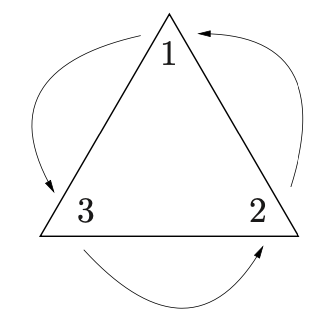
\includegraphics[scale=0.4]{dihedralgroups}
\caption{Example of an equilateral triangle as a Dihedral Group $D_6$}
\end{figure}

\begin{remark}
The properties of dihedral groups are as follows:
\begin{enumerate}[label=(\roman*)]
\setlength{\itemsep}{0pt}
\item $\abs{r}=n$, as $1, r, \ldots, r^n$ are all distint, and $r^n = 1$
\item $\abs{s}=2$, as $s^2 = 1$
\item $s \neq r^i$ for any $i$
\item $sr^i \neq sr^j$ for all $0 \leq i, j \leq n-1$, with $i \neq j$\\
Hence $D_{2n} = \{1,r,r^2,\ldots, r^{n-1}, s, sr, sr^2, \ldots, sr^{n-1}\}$.\\
Each element can be written uniquely in the form $s^k r^i$ for $k \in {0,1}$, $0\leq i \leq n-1$.
\item $rs=sr^{-1}$. Hence $r$ and $s$ do not commute, and $D_{2n}$ is non-abelian.
\item $r^i s = sr^{-i}$ for all $0\leq i \leq n$
\end{enumerate}
\end{remark}

\subsubsection{Symmetric Groups}

\begin{definition}
Let $\Omega$ be any nonempty set, and $S_{\Omega}$ be the set of all bijections from $\Omega$ to itself (the set of all permutations of $\Omega$. Then the set $S_{\Omega}$ is a group under function composition $\circ$.\\
The identity of $S_{\Omega}$ is the permutation $1$ defined by $1(a)=a \ \forall a\in \Omega$.\\
For every permutation $\sigma: \Omega \rightarrow \Omega$ there is a $2$-sided inverse function $\sigma^{-1}: \Omega \rightarrow \Omega$ satisfying $\sigma \circ \sigma^{-1} = \sigma^{-1} \circ \sigma = 1$. Thus all group axioms hold for $(S_{\Omega}, \circ)$, the \hlt{symmetric group on the set $\Omega$}.\\
The elements of $S_{\Omega}$ are the permutations of $\Omega$, not elements of $\Omega$ itself.\\
If $\Omega = \{1,2,\ldots, n\}$ is a finite set, then $S_n$ is the \hlt{symmetric group of degree $n$}.
\end{definition}

The group $S_n$ plays an important role as a means of illustrating and motivating the general theory.

\begin{theorem}
The order of $S_n$ is $n!$.
\end{theorem}
\begin{proof}
The permutations of $\{1,2,\ldots, n\}$ are precisely the injective functions of this set to itself as it is finite. We count the number of injective functions. For $\sigma(n)$, this is precisely $n \cdot (n-1) \cdot (n-2) \cdots 2 \cdot 1 = n!$ possible injective functions from $\{1,2,\ldots, n\}$ to itself.
\end{proof}

We now introduce the notation for writing elements $\sigma$ of $S_n$ with cycle decomposition.

\begin{definition}
A \hlt{cycle} is a string of integers which represents the elements of $S_n$ which cyclically permutes these integers and fixes other integers.\\
The cycle $(a_1 \ a_2 \ \cdots \ a_m)$ is the permutation which sends $a_i$ to $a_{i+1}$, $1 \leq i \leq m-1$ and sends $a_m$ to $a_1$.\\
In general, for each $\sigma \in S_n$, the numbers from $1$ to $n$ will be rearranged and grouped into $k$ cycles of the form
\begin{equation}
(a_1 \ a_2 \ \cdots \ a_{m_1})(a_{m_1 + 1} \ a_{m_1 +2} \ \cdots \ a_{m_2}) \cdots (a_{m_{k-1} + 1} \ a_{m_{k-1} + 2} \ \cdots \ a_{m_k}) \nonumber
\end{equation}
\end{definition}

\begin{remark}
In Cauchy's two line notation, the natural order of elements of $\Omega$, say $x_1, x_2, \ldots, x_n$ is listed in the first row, then the images of each element in the second row.
\begin{equation}
\sigma = 
\begin{pmatrix}
x_1 & x_2 & \cdots & x_n \\
\sigma(x_1) & \sigma(x_2) & \cdots & \sigma(x_n)
\end{pmatrix} \nonumber
\end{equation}
We may omit the first row and write the permutation in one-line notation as:
\begin{equation} 
\begin{pmatrix}
\sigma(x_1) & \sigma(x_2) & \cdots & \sigma(x_n)
\end{pmatrix} \nonumber
\end{equation}
\end{remark}

\begin{definition}
The \hlt{length} of a cycle is the number of integers which appear in it.\\
A cycle of length $t$ is called a \hlt{$t$-cycle}.\\
Two cycles are \hlt{disjoint} if they have no numbers in common.\\
The inverse permutation is given by reversing the order of elements in the permutation's cycles.
\end{definition}

\begin{algorithm}
The \hlt{cycle decomposition algorithm} is as follows:
\begin{enumerate}[label=\arabic*.]
\setlength{\itemsep}{0pt}
\item Write an opening bracket then select an arbitrary element $x$ of $\Omega$ and write it down: $(x$
\item Trace the orbit of $x$, write down its values over successive applications of $\sigma$: $(x \ \sigma(x) \ \sigma(\sigma(x)) \cdots$
\item Repeat until the value returns to $x$ and write a closing parenthesis rather than $x$: $(x \ \sigma(x) \ \sigma(\sigma(x)) \cdots)$
\item Now continue with an element $y$ of $\Omega$ not yet written down, and proceed in the same way: $(x \ \sigma(x) \ \sigma(\sigma(x)) \cdots)(y \cdots)$
\item Repeat until all elements of $\Omega$ are written in cycles.
\end{enumerate}
\end{algorithm}

\subsubsection{Matrix Groups}

Matrix groups have coefficients that come from fields. A field is the smallest mathematical structure which all arithmetic operations $(+, -, \times, \div)$ (division by nonzero elements) can be performed.

\begin{definition}
A \hlt{field} is a set $F$ with two binary operations $+, \cdot$ on $F$ such that $(F, +)$ is an abelian group (with identity $0$), and $(F-\{0\}, \cdot)$ is also an abelian group. The following distributive law holds:
\begin{equation}
a\cdot (b+c) = (a \cdot b) + (a \cdot c), \forall a,b,c \in F \nonumber
\end{equation}
For any field $F$, let $F^{\times} = F - \{0\}$
\end{definition}

\begin{definition}
A \hlt{matrix group} is a group $G$ consisting of invertible matrices over a field $K$, with the operation of matrix multiplication.\\
The \hlt{general linear group} of degree $n$ is the set of $n \times n$ invertible matrices with matrix multiplication, denoted $GL_n(\F)$. If $n \geq 2$, then the group $GL_n(\F)$ is not abelian.\\
The \hlt{special linear group} is a subgroup of $GL_n(\F)$, consisting of matrices with determinant $1$, denoted $SL_n(\F)$.
\end{definition}

We dive deeper into the results in Modules and Vector Spaces in Section \ref{sect:modandvec}.

\subsubsection{The Quaternion Group}

\begin{definition}
The \hlt{quaternion group} is defined by $Q_8 = \{1, -1, i, -i, j, -j, k, -k\}$, with product $\cdot$ computed as follows:
\begin{alignat*}{2}
1 \cdot a &= a \cdot 1 = a &&\forall a \in Q_8 \nonumber \\
(-1) \cdot (-1) = 1,\ \ &(-1) \cdot a = a \cdot (-1) = -a \ \ \ \ &&\forall a \in Q_8 \nonumber \\
i \cdot i &= j \cdot j = k \cdot k= -1 \nonumber \\
i \cdot j &= k, \ \ \ \ \ \ \ j \cdot i = -k \nonumber \\
j \cdot k &= i, \ \ \ \ \ \ \ k \cdot j = -i \nonumber \\
k \cdot i &= j, \ \ \ \ \ \ \ i \cdot k = -j \nonumber
\end{alignat*}
Note that $Q_8$ is a non-abelian group of order 8.
\end{definition}

\begin{figure}[H]
\centering
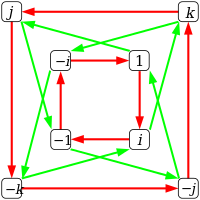
\includegraphics[scale=0.4]{quaterniongroup}
\caption{The Cayley diagram of the Quaternion Group $Q_8$.}
\end{figure}

\subsubsection{Homomorphism and Ismomorphism}

We define what makes two group 'look the same', i.e., having exactly the same group-theoretic structure (an isomorphism) in this section.

\begin{definition}
Let $(G, *), (H, \diamond)$ be groups. A map $\varphi: G \rightarrow H$ such that
\begin{equation}
\varphi(x*y) = \varphi(x) \diamond \varphi(y), \ \ \forall x,y \in G \nonumber
\end{equation}
is a \hlt{homomorphism}.
\end{definition}

If the group operations for $G, H$ are not explicitly written, then this is simply $\varphi(xy) = \varphi(x) \varphi(y)$, but the product $xy$ on the left is computed in $G$, while the product $\varphi(x) \varphi(y)$ is computed in $H$.\\
Intuitively, a map $\varphi$ is a homomorphism if it respects the group structures of its domains and codomains.

\begin{definition}
The map $\varphi: G \rightarrow H$ is a \hlt{isomorphism} and $G$ and $H$ are \hlt{isomorphic}, denoted $G \cong H$, if:
\begin{enumerate}[label=(\roman*)]
\setlength{\itemsep}{0pt}
\item $\varphi$ is a homomorphism (i.e., $\varphi(xy) = \varphi(x) \varphi(y)$), and
\item $\varphi$ is a bijection.
\end{enumerate}
\end{definition}

Intuitively, $G$ and $H$ are the same group, except the elements and operations may be written different in $G$ and $H$. Thus, any property which $G$ has which only depends on group structure of $G$ also holds for $H$.

\begin{definition}
Let $\mathscr{G}$ be any nonempty collection of groups. Then the relation $\cong$ is an equivalent relation on $\mathscr{G}$, and the equivalence classes are called \hlt{isomorphism classes}.
\end{definition}

\begin{example}{\color{white}space}
\begin{enumerate}[label=(\roman*)]
\setlength{\itemsep}{0pt}
\item For any group $G$, $G \cong G$, the identity map.
\item The exponential map $\exp : \R \rightarrow \R^+$, defined by $\exp(x)=e^x$, is an isomorphism from $(\R, +)$ to $(\R^+, \times)$
\end{enumerate}
\end{example}

\begin{figure}[H]
\centering
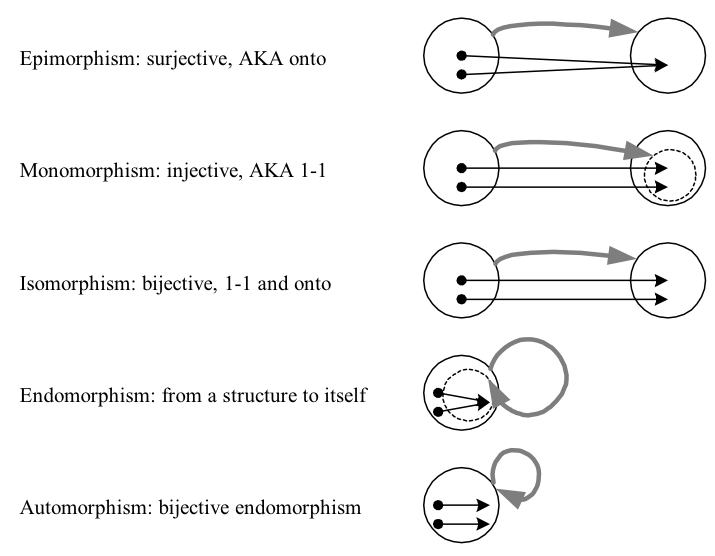
\includegraphics[scale=0.8]{comparisonofmorph}
\caption{Comparison of all types of morphism.}
\end{figure}

\subsubsection{Group Actions}

Group action is a powerful tool for proving theorems for abstract groups, and for unravelling the structure of the groups. This is a method for studying an algebraic object by seeing how it can act on other structures.

\begin{definition}
A \hlt{(left) group action} of a group $G$ on a set $A$ is a map from $G \times A$ to $A$, written as $g \cdot a \ \forall g\in G$ and $a\in A$, satisfying the following properties:
\begin{enumerate}[label=(\roman*)]
\setlength{\itemsep}{0pt}
\item $g_1 \cdot (g_2 \cdot a) = (g_1 g_2) \cdot a$ $\forall g_1, g_,2 \in G$ and $a \in A$, and
\item $1 \cdot a = a$ $\forall a \in A$
\end{enumerate}
A \hlt{right group action} is similarly defined, with group elements on the right of set elements.\\
Hence, for each fixed $g\in G$, we get a map $\sigma_g$ defined by:
\begin{align}
\sigma_g : A &\rightarrow A \nonumber \\
\sigma_g(a) &= g \cdot a \nonumber
\end{align}
\end{definition}

\begin{proposition}{\color{white}space}
\begin{enumerate}[label=(\roman*)]
\setlength{\itemsep}{0pt}
\item For each $g\in G$, $\sigma_g$ is a permutation of $A$, and
\item the map from $G$ to $S_A$ defined by $g \mapsto \sigma_g$ is a homomorphism
\end{enumerate}
\end{proposition}
\begin{proof}{\color{white}space}
\begin{enumerate}[label=(\roman*)]
\setlength{\itemsep}{0pt}
\item To show that $\sigma_g$ is a permutation of $A$, we show that as a set map from $A$ to $A$, it has a $2$-sided inverse $\sigma_{g^{-1}}$. For all $a \in A$: 
\begin{alignat*}{2}
(\sigma_{g^{-1}} \circ \sigma_g)(a) &= \sigma_{g^{-1}}(\sigma_g(a)) \ \ \ && \textnormal{(by definition of function composition)} \\
&= g^{-1} \cdot(g\cdot a) && \textnormal{(by definition of $\sigma_{g^{-1}}$ and $\sigma_g$)} \\
&= (g^{-1} g)\cdot a && \textnormal{(by property (1) of an action)} \\
&= 1 \cdot a = a && \textnormal{(by property (2) of an action)}
\end{alignat*}
Hence, $\sigma_{g^{-1}} \circ \sigma_{g}$ is the identity map from $A$ to $A$, with a $2$-sided inverse. Since $g$ is arbitrary, we may interchange the roles of $g$ and $g^{-1}$ to obtain $\sigma_{g} \circ \sigma_{g^{-1}}$, which is also the identity map on $A$. Hence $\sigma_{g}$ has a $2$-sided inverse, hence is a permutation of $A$.
\item let $\varphi: G \rightarrow S_A$ be defined by $\varphi(g) = \sigma_g$. Note that (i) has shown that $\sigma_g$ is indeed an element of $S_A$. To see that $\varphi$ is a homomorphism, we must prove $\varphi(g_1 g_2) = \varphi(g_1) \circ \varphi(g_2)$. For all $a\in A$:
\begin{alignat*}{2}
\varphi(g_1 g_2)(a) &= \sigma_{g_1 g_2} (a) \ \ \ && \textnormal{(by definition of $\varphi$)} \\
&= (g_1 g_2) \cdot a && \textnormal{(by definition of $\sigma_{g_1 g_2}$)} \\
&= g_1 \cdot (g_2 \cdot a) && \textnormal{(by property (1) of an action)} \\
&= \sigma_{g_1}(\sigma_{g_2} (a)) && \textnormal{(by definition of $\sigma_{g_1}$ and $\sigma_{g_2}$)} \\
&= (\varphi(g_1) \circ \varphi(g_2)) (a) \ \ && \textnormal{(by definition of $\varphi$)}
\end{alignat*}
\end{enumerate}
\end{proof}

\begin{definition}
The \hlt{permutation representation} associated to the group action is the homomorphism from $G$ to $S_A$. Let $\varphi: G \rightarrow S_A$ be any homomorphism from a group $G$ to the symmetric group on a set $A$, then the map $G \times A \mapsto A$ is defined by
\begin{equation}
g \cdot a = \varphi(g)(a) \ \ \forall g\in G, \a \in A \nonumber
\end{equation}
\end{definition}

\begin{definition}
Let $ga=a$ for all $g\in G, a\in A$. Then this is the \hlt{trivial action}, and $G$ is said to \hlt{act trivially} on $A$. The distinct elements of $G$ induce the same permutation on $A$. The associated permutation representation $G\rightarrow S_A$ is the trivial homomorphism which maps every element of $G$ to the identity.
\end{definition}

\begin{definition}
If $G$ acts on a set $B$ and distinct elements of $G$ induce distinct permutations of $B$, then the action is \hlt{faithful}. The associated permutation representation is injective.\\
The \hlt{kernel} of the action $G$ on $B$ is $\ker = \{g \in G \ \vert \ gb = b \ \forall b \in B \}$.
\end{definition}

\subsection{Subgroups}

To study the structure of a group, a basic method is to study quotients of an object (to collapse a group into a smaller group).

\subsubsection{Centralisers, Normalisers, Stabilisers, Kernels}

\begin{definition}
Let $G$ be a group. The subset $H$ of $G$ is a \hlt{subgroup} of $G$ if $H$ is nonempty and $H$ is closed under products and inverses. If $H$ is a subgroup of $G$, this is denoted $H \leq G$.
\end{definition}

\begin{example}{\color{white}space}
\begin{enumerate}[label=(\roman*)]
\setlength{\itemsep}{0pt}
\item $\Z \leq \Q$, and $\Q \leq \R$ with the operation of addition.
\item Any group $G$ has two subgroups: $H = G$, and $H = \{1\}$ (the \hlt{trivial subgroup}).
\item If $H \leq G$ and $K \leq H$, then $H \leq G$ by transitivity property.
\end{enumerate}
\end{example}

\begin{proposition}
\hlt{(The Subgroup Criterion)}
\end{proposition}

\subsection{Quotient Groups, Homomorphisms}

\subsection{Group Actions}

\subsection{Direct and Semidirect Products, Abelian Groups}

This section introduces methods to construct larger groups from smaller ones with direct and semidirect product. This then allow us to completely classify all finite abelian groups with the Fundamental Theorem on Finitely Generated Abelian Groups.

\subsubsection{Direct Products}

\begin{definition}
The \hlt{direct product} $G_1 \times G_2 \times \cdots$ of groups $G_1, G_2, \ldots$ with operations $*_1, *_2, \ldots$ is the set of sequences $(g_1, g_2, \ldots)$ where $g_i \in G_i $, with operation defined component-wise:
\begin{equation}
(g_1, g_2, \ldots) * (h_1, h_2, \ldots) = (g_1 *_1 h_1, g_2 *_2 h_2, \ldots) \nonumber
\end{equation}
\end{definition}

\begin{example}{\color{white}space}
\begin{enumerate}[label=(\roman*)]
\setlength{\itemsep}{0pt}
\item Let $G_i = \R$ for $i = 1,2,\ldots,n$. Then $\R \times \R \times \cdots \times \R$ ($n$-factors) is the Euclidean $n$-space $\R^n$ with vector addition $(a_1, a_2, \ldots, a_n) + (b_1, b_2, \ldots, b_n) = (a_1 + b_1, a_2 + b_2, \ldots, a_n + b_n)$
\item For groups forming direct product, let $G_1 = \Z, G_2 = S_3, G_3 = GL_2(\R)$, where the group operations are addition, composition, and matrix multiplication. Then the operation $G_1 \times G_2 \times G_3$ is defined to be
\begin{equation}
(n,\sigma, \begin{pmatrix}
a & b \\
c & d
\end{pmatrix})
(m,\tau, \begin{pmatrix}
p & q \\
r & s
\end{pmatrix}) =
(n+m,\tau \circ \sigma, \begin{pmatrix}
ap+br & aq+bs \\
cp+dr & cq+ds
\end{pmatrix}) \nonumber
\end{equation}
\end{enumerate}
\end{example}

\begin{proposition}
If $G_1, \ldots, G_n$ are groups, then their direct product is a group of oder $\abs{G_1} \abs{G_2} \cdots \abs{G_n}$. If any $G_i$ is infinite, so is the direct product.
\end{proposition}
\begin{proof}
Let $G = G_1 \times G_2 \times \cdots \times G_n$.\\
The group axioms hold for $G$ since each axiom is a consequence of the fact that the same axiom in Proposition \ref{prop:proofgroupop} holds in each factor $G_i$, and the operation on $G$ is defined component-wise. \\
The identity of $G$ is the $n$-tuple $(1_1, 1_2, \ldots, 1_n)$, where each $1_i$ is the identity of $G_i$.\\
The inverse of $(g_1, g_2, \ldots, g_n)$ is $(g_1^{-1}, g_2^{-1}, \ldots, g_n^{-1})$, where each $g_i^{-1}$ is the inverse of $g_i$ in $G$.\\
Hence the formula for the order of $G$ is clear.
\end{proof}

Rearranging factors of the direct product results in a direct product isomorphic to the original one.

\begin{proposition}
Let $G_1, G_2, \ldots, G_n$ be groups, and let $G = G_1 \times \cdots \times G_n$ be their direct product.
\begin{enumerate}[label=(\roman*)]
\setlength{\itemsep}{0pt}
\item For each fixed $i$, the set of elements of $G$ which have the identity of $G_j$ in the $j^{\textnormal{th}}$ position for all $j \neq i$ and the arbitrary elements of $G_i$ in position $i$ is the subgroup of $G$ isomorphic to $G_i$:
\begin{equation}
G_i \cong \{(1,1,\ldots, 1, g_i, 1, \ldots, 1) \ \vert \ g_i \in G_i\} \textnormal{ (where $g_i$ is at the $i^{\textnormal{th}}$ position)} \nonumber
\end{equation}
If we identify $G_i$ with this subgroup, then $G_i \trianglelefteq G$ and
\begin{equation}
G/G_i \cong G_1 \times \cdots \times G_{i-1} \times G_{i+1} \times \cdots \times G_n \nonumber
\end{equation}
\item For each fixed $i$, define $\pi_i: G \rightarrow G_i$ by
\begin{equation}
\pi_i((g_1 ,g_2, \ldots, g_n)) = g_i \nonumber
\end{equation}
Then $\pi_i$ is a surjective homomorphism with
\begin{align}
\ker{\pi_i} &= \{(g_1, \ldots, g_{i-1}, 1, g_{i+1}, \ldots, g_n)\ \ \vert \ g_j\in G_j \ \forall j\neq i\}\nonumber \\
&\cong G_1 \times \cdots \times G_{i-1} \times G_{i+1} \times \cdots \times G_n \nonumber
\end{align}
where $1$ appears at position $i$. 
\item Under the identifications in part (i), if $x \in G$ and $y \in G_j$ for some $i\neq j$, then $xy = yx$
\end{enumerate}
\end{proposition}

\subsection{Further Topics in Group Theory}

\subsubsection{$p$-groups, Nilpotent Groups, Solvable Groups}




\newpage

\section{Ring Theory}

\subsection{Basic Axioms}

\begin{definition}
A \hlt{ring} is a nonempty set $ R $ with two binary operations $ + $ (addition) and $ \times $ (multiplication), $ (R, +, \times) $, such that:
\begin{enumerate}[label=(\roman*)]
\item $(R, +)$ is an additive abelian group with $0$ as the additive identity
\item the binary operation $\times$ is associative: 
\begin{equation}
(a \times b) \times c = a \times (b \times c), \ \forall a, b, c \in R
\nonumber
\end{equation}
\item left and right distributive laws: 
\begin{align}
(a+b) \times c &= (a \times c) + (b \times c) \ \forall a, b, c \in R \nonumber \\
a \times (b+c) &= (a \times c) + (b \times c), \ \forall a, b, c \in R \nonumber
\end{align}
\end{enumerate}
If in addition, $a \times b = b \times a \ \forall a, b \in R$, then $R$ is a \hlt{commutative ring}.
\end{definition}


\begin{definition}
The ring $R$ has a \hlt{multiplicative identity} if there is an element $1_R \in R$ such that 
\begin{equation}
1_R \times a = a \times 1_R = a, \ \forall a \in R
\nonumber
\end{equation}
The ring $R$ has a \hlt{additive identity} if there is an element $0_R \in R$ such that 
\begin{equation}
a-b = a+(-b) = 0_R
\nonumber
\end{equation}
where $-b$ is the \hlt{additive inverse}.
\end{definition}


\begin{definition}
A \hlt{division ring} $R$ is a ring such that:
\begin{enumerate}[label=(\roman*)]
\item $R$ has a multiplicative identity $1_R$;
\item $1_R \neq 0_R$; and
\item $\forall$ nonzero element $a \in R \textbackslash \{0\}$ has a unique multiplicative inverse $a \textsuperscript{-1}$ such that
\begin{equation}
aa \textsuperscript{-1} = 1 = a \textsuperscript{-1} a
\nonumber
\end{equation}
\end{enumerate}
\end{definition}


\begin{definition}
A \hlt{field} is a division ring which is commutative.\\
If $R$ is a division ring (field), then $(R, \times)$ is a (commutative) \hlt{multiplicative group}, $R^\times = R \textbackslash \{0\}$.\\
\end{definition}


\begin{definition}
Let $F = (F, +, \times) $ be a field. A nonempty subset $E \subseteq F$ is a \hlt{subfield} if:
\begin{enumerate}[label=(\roman*)]
\item $(E, +)$ is an additive subgroup of $(F, +)$;
\item $E$ is closed under multiplication $\times$: $a, b \in E \Rightarrow a \times b \in E$;
\item $1_F \in E$; and
\item $a \in E \textbackslash \{0\} \Rightarrow a \textsuperscript{-1} \in E$
\end{enumerate}
\end{definition}


\begin{remark}
The \hlt{trivial ring} is $\{0\}$.\\
The \hlt{integer ring} is $(\mathbb{Z}, +, \times )$ with $ 1 $, but is neither a division ring or field.\\
$n \mathbb{Z} = \{ns | s \in \mathbb{Z}\} $ is a subring of $\mathbb{Z}$.\\
$(\mathbb{Z} / n \mathbb{Z}, +, \times) $ is a commutative ring with $ 1 $ for $ n \geq 2 $.\\
\end{remark}


\begin{remark}
The $2$-dimensional vector space 
\begin{equation}
\mathbb{Q}[\sqrt{D}] = \mathbb{Q} + \mathbb{Q}\sqrt{D} = \{a+b\sqrt{D}|a, b \in \mathbb{Q} \}
\nonumber
\end{equation}
with $\mathbb{Q}$-basis $\{1, \sqrt{D} \}$ is a \hlt{Quadratic Field}.\\
Define $\mathbb{Q}(\sqrt{D}) = \{ \frac{ a+b\sqrt{D} }{ c+d\sqrt{D} } | a, b, c, d \in \mathbb{Q}, c + d\sqrt{D} \neq 0 \} $. \\
Then $\mathbb{Q}(\sqrt{D}) = \mathbb{Q}[\sqrt{D}]$.\\
More generally, for a field $F$, 
\begin{equation}
\mathbb{Q}(F) = \{\frac{\alpha}{\beta} = \alpha \beta \textsuperscript{-1} |\ \alpha \beta , \in F, \beta \neq 0\} = F
\nonumber
\end{equation}
\end{remark}


\begin{remark}
Let $H=\mathbb{R} + \mathbb{R} i + \mathbb{R} j + \mathbb{R} k = \{a+bi+cj+dk|a,b,c,d \in \mathbb{R}\}$ be the $4$-dimensional vector space over $\mathbb{R}$ with $\mathbb{R}$-basis $(1, i, j, k)$.\\
The multiplication is extended linearly by distributive law: 
\begin{align}
i^2 = j^2 = k^2 = -1 \nonumber \\
ij=k=-ji \nonumber \\
jk=i=-kj \nonumber \\
ki=j=-ik \nonumber
\end{align}
Then $H$ is a \hlt{Real Quaternion Ring}.\\
The \hlt{Rational Hamilton Quaternion Ring} is:
\begin{equation}
H_\mathbb{Q}=\mathbb{Q}+\mathbb{Q}i+\mathbb{Q}j+\mathbb{Q}k=\{a+bi+cj+dk|\ a, b, c, d\in \mathbb{Q}\} \nonumber
\end{equation}
\end{remark}


\begin{remark}
Let $\mathbb{R}V[x]=\{f:\mathbb{R}\rightarrow\mathbb{R}\}$ be the set of all real-valued functions.\\
Let $x\mapsto c(x) = c$ be a constant function.\\
For $f, g \in \mathbb{R}V[x]$, the natural addition is
\begin{equation}
x\mapsto (f+g)(x) = f(x)+g(x) \nonumber
\end{equation}
The multiplication (not composition) is 
\begin{equation}
x\mapsto (fg)(x)=f(x)g(x) \nonumber
\end{equation}
$(\mathbb{R}V[x], +, \times)$ is a commutative \hlt{(real valued-function) ring} with multiplicative identity $1$ being the constant function $1$.\\
\end{remark}


\begin{definition}
Let $R$ be a ring with $1 \neq 0$. An element $u \in R$ is a \hlt{unit} if it has a multiplicative identity inverse $u'$ such that $uu'=1=u'u$.\\
The \hlt{set of all units} of $R$ are 
\begin{equation}
U(R)=\{u\in R | u \ is \ a \ unit\} \nonumber
\end{equation}
The \hlt{multiplicative group of units of the ring} $R$ is $(U(R), \times)$.\\
\end{definition}


\begin{remark}
More generally, let $X$ be a set and $R$ be a ring. Let $X \textsubscript{to} R := \{f: X \rightarrow R\}$ be the set of all maps between $X$ and $R$. Then for $f, g \in X \textsubscript{to} R $, there are natural addition $f+g$ and multiplication $fg$ ($x\mapsto f(x)g(x)$).\\
Then $(X \textsubscript{to} R, +, \times)$ is a ring, called the \hlt{$R$-Valued Function Ring}.\\
If $R$ has $1$ then so does $X \textsubscript{to} R$. If $R$ is commutative then so does $X \textsubscript{to} R$.\\
Every $c\in R$ defines a constant function (an element in $X \textsubscript{to} R$)
\begin{align}
c:X &\rightarrow R \nonumber \\
x &\mapsto c(x)=c \nonumber
\end{align}
Identify $R$ with the subset of $X \textsubscript{to} R$ of constant function. Then $R$ is a subring of $X \textsubscript{to} R$.\\
\end{remark}


\begin{remark}
Let $n \geq 2$. Then $U(\mathbb{Z}/n\mathbb{Z})$ is a commutative multiplicative group of order 
\begin{equation}
\left| U(\mathbb{Z}/n\mathbb{Z}) \right| = \varphi (n) \nonumber
\end{equation}
Hence $\varphi (n)$ is the \hlt{Euler's $\varphi$-function}, 
\begin{equation}
\varphi (n)=\left|\{1 \leq s \leq n | gcd(s, n) = 1\}\right| \nonumber
\end{equation}
\end{remark}


\begin{definition}
An \hlt{Integral Domain} is a commutative ring with $1\neq 0$ such that $\forall a, b, \in R, \ ab = 0 \Rightarrow a=0 \ or \ b=0$,
or equivalently, $\forall a, b \in R, \ a \neq 0, \ b \neq 0 \Rightarrow ab \neq 0$.\\
$\mathbb{Z}$ is an integral domain.\\
Every field is an integral domain.\\
\end{definition}


\begin{definition}
Let $R$ be a ring. A nonzero element $a \in R$ is a 	\hlt{zero divisor} if there is a nonzero $b\in R$ such that either $ab=0$ or $ba=0$.\\
A commutative ring $R$ with $1$ is an integral domain if and only if $R$ as no zero divisors.\\
\end{definition}


\begin{proposition}
Let $R$ be a ring with $1 \neq 0$. $R$ is an integral domain if and only if cancellation law holds: 
\begin{equation}
\forall a, b, c \in R, \ c \neq 0, \ ca=cb \Rightarrow a=b \nonumber
\end{equation}
\end{proposition}


\begin{corollary}
Let $R$ be a finite integral domain, i.e., $R$ is an integral domain with the cardinality $\left| R \right| < \infty$. Then $R$ is a field.\\
\end{corollary}


\begin{proposition}
Let $n \geq 2$. Then the following are equivalent:
\begin{enumerate}[label=(\roman*)]
\item $\mathbb{Z}/n\mathbb{Z}$ is a field
\item $\mathbb{Z}/n\mathbb{Z}$ is an integral domain
\item $n$ is a prime
\end{enumerate}
\end{proposition}


\begin{definition}
Let $R$ be a ring. A nonempty subset $S \subseteq R$ is a \hlt{subring} of $R$ if:
\begin{enumerate}[label=(\roman*)]
\item $(S, +)$ is an additive subgroup of $(R, +)$ and
\item $S$ is closed under multiplication
\end{enumerate}
\begin{equation}
\mathbb{Z} \subset \mathbb{Q} \subset \mathbb{R} \subset \mathbb{C} \nonumber
\end{equation}
\end{definition}


\begin{proposition}
\hlt{(Subring Criterion)} Let $R$ be a ring and $S \subseteq R$ a nonempty subset. \\
Then the following are equivalent:
\begin{enumerate}[label=(\roman*)]
\item $S$ is a subring of $R$
\item $S$ is closed under subtracting and multiplication:
\begin{align}
a,b\in S &\Rightarrow ab\in S \nonumber \\
a-b &= a + (-b) \in S \nonumber
\end{align}
\end{enumerate}
\end{proposition}


\begin{remark}
Being a subring is a transitive condition. If $R$ is a subring of $S$ and $S$ is a subring of $T$, then $R$ is a subring of $T$.\\
If both $S_i$ are subring of $R$ and $S_1 \subseteq S_2$, then $S_1$ is a subring of $S_2$.\\
\end{remark}


\begin{remark}
\hlt{(Subring without 1)} If $R$ is a ring with $1 = 1_R$ then a subring $S \subseteq R$ may not contain $1$, i.e., $m\mathbb{Z} = {ms|s\in \mathbb{Z}, \left| m \right| \geq 2}$ is a subring of $\mathbb{Z}$ which does not contain $1$.
\end{remark}


\begin{remark}
\hlt{(Intersection of subrings)} Let $R_\alpha$ ($\alpha \in \Sigma$) be a (not necessarily finite or countable) collection of subrings of a ring $R$. Then the intersection $\bigcap\limits_{\alpha \in \Sigma} R_\alpha$ is a subring of $R$.\\
Generally, the union of subrings may not be a subring.\\
\end{remark}


\begin{remark}
\hlt{(Union of ascending subrings)} Let $R_1 \subseteq R_2 \subseteq \cdots $ be an ascending chain of subrings $R_i$ of a ring $R$.
Then the union $\bigcup\limits_{i=1}^{\infty} R_\alpha$ is a subring of $R$.\\
\end{remark}


\begin{remark}
\hlt{(Addition of subrings)} Let $R$ be a ring and let $R_i$ be subrings of $R$.\\
Then the addition $R_1 + \cdots + R_n$ is closed under subtraction, but may not be closed under multiplication, hence may not be a subring of $R$.\\
\end{remark}


\begin{remark}
\hlt{(Integral domain is a subring of a field)}\\
Let $F$ be a field. Let $R \subseteq F$ be a subring such that $1 \in R$. Then $R$ is an integral domain.\\
Every integral domain $R$ is a subring of some field $\mathbb{Q}(R)$ (the fractional field of $R$).\\
\end{remark}


\begin{remark}
\hlt{(Product of Rings)} let $n \geq 1$ and let $R_i = (R_i, +, \times)$ ($i=1, \ldots, n$) be rings.\\
Then the direct product is a ring, 
\begin{align}
R &= R_1 \times \cdots \times R_n \nonumber \\
(a_1, \ldots, a_n) &\times (a'_1, \ldots, a'_n) = (a_1 a'_1, \ldots, a_n a'_n) \nonumber
\end{align}
The unit subgroups has the relation 
\begin{equation}
U(R) = U(R_1)\times \cdots \times U(R_n) \nonumber
\end{equation}
\end{remark}


\subsection{Examples of Rings}

\begin{definition}
The \hlt{polynomial ring $R[x]$ over a ring $R$} is $(R[x], +, \times)$,  where 
\begin{equation}
R[x] = \{\sum_{j=0}^{d} b_j x_j | d \geq 0, \ b_j \in \mathbb{R} \} \nonumber
\end{equation}
There are natural addition and multiplication operations for polynomials.\\
\end{definition}


\begin{remark}
Let $R$ be a commutative ring with $1$. Let $S:= R[x]$ be the polynomial ring over $R$.
\begin{enumerate}[label=(\roman*)]
\item $R$ is a subring of $S$ which consists of constant polynomial functions.
\item $0_S = 0_R$
\item $S$ contains $1=1_S$, and $1_S = 1_R$.
\end{enumerate}
\end{remark}


\begin{proposition}
\hlt{(Polynomial ring over integral domain)} Let $R$ be an integral domain. Let $f(x), g(x) \in R[x]$. Then
\begin{enumerate}[label=(\roman*)]
\item $\degs(f(x)g(x)) = \degs(f(x)) + \degs(g(x))$
\item $U(R[x]) = U(R)$. Namely, $g(x)$ is a unit of $R[x]$ if and only if $g=a_0 \in R$ (constant polynomial) with $a_0$ a unit in $R$.
\item $R[x]$ is an integral domain
\end{enumerate}
\end{proposition}


\begin{remark}
The {{\color{blue} matrix ring of $n \times n$ square matrices with entries in the ring $R$}} is defined as $(M_n(R), +, \times)$, where\\
$M_n(R) = \left\{A=\begin{pmatrix}
a_{11} & a_{12} & \cdots & a_{1n}\\
a_{21} & a_{22} & \cdots & a_{2n}\\
\vdots & \vdots & \ddots & \vdots\\
a_{m1} & a_{m2} & \cdots & a_{mn}\\
\end{pmatrix} | a_{ij} \in R \right\}$\\
If $A = (a_{ij}), B = (b_{ij}) \in M_n(F)$, then $A+B=(a_{ij} + b_{ij}), AB = (c_{ij})$ where $c_{ij} = \sum_{k=1}^{n} a_{ik} b_{kj}$.\\
$A=(a_{ij}) = Diag[a_{11}, \ldots, a_{nn}]$ is a diagonal matrix if $a_{ij} = 0$ ($i \neq j$).\\
$A=(a_{ij}) = Diag(a_1, \ldots, a_n)$ is a scalar matrix if $a_{ii} = a \in R \ \forall i$, and $a_{ij} = 0$ ($i \neq j$).\\
$A=(a_{ij})$ is an upper triangular matrix if $a_{ij}=0$ ($i < j$). The lower triangular matrix is defined similarly.\\
\end{remark}


\begin{remark}
Let $R$ be a ring and $S = M_n(R)$ the matrix ring with entries in $R$. Then
\begin{enumerate}[label=(\roman*)]
\item $0_S=(a_{ij})$ where $a_{ij} = 0$ (the zero matrix)
\item If $R$ has $1 = 1_R$, then $S$ also has $1 = 1_S$ with $1_S = Diag[1_R, \ldots, 1_R]$
\item The set $S_{c_n}(R) = \{Diag[a, \ldots, a] | a_i \in R\}$ of all scalar matrices in $M_n(R)$ is a subring of $M_n(R)$. There is a natural ring isomorphism $R \cong S_{c_n}(R)$.
\item The set $D_n(R) = \{Diag[a_1, \ldots, a_n] | a_i \in R\}$ of all diagonal matrices in $M_n(R)$ is a subring of $M_n(R)$. There is a natural ring isomorphism $D_n(R) \cong R^n := R \times \cdots \times R $ ($n$ times).
\item The set $UT_n(R):= \{(a_{ij} | (a_{ij} \in R, (a_{ij} = 0 (\forall \ i > j))\}$ of all upper triangular matrices in $M_n(R)$ is a subring of $M_n(R)$. Similarly, the set $LT_n(R)$ of all lower triangular matrices in $M_n(R)$ is a subring of $M_n(R)$.
\item If $R$ is a subring of $R$, then $M_n(T)$ is a subring of $M_n(R)$
\item Even if $R$ is commutative, $M_n(R)$ may not be commutative when $n \geq 2$.
\item If $n \geq 2$, then $M_n(R)$ is not an integral domain (even when $R$ is a field).
\end{enumerate}
\end{remark}


\begin{definition}
Let $R$ be a ring with $1$. Set $GL_n(R) := U(M_n(R))$ the set of all units in $M_n(R)$. Then $GL_n(R)$ is a multiplicative group called the \hlt{general linear group of degree $n$ over $R$}.
\end{definition}


\begin{definition}
Let $R$ be a commutative ring with $1$. Define determinant $det(A) = \left| A \right|$, Let $SL_n(R) := \{A \in M_n(R) | det(A) = 1\}$ be the set of all matrices in $M_n(R)$ with determinants equal to $1$. \\
Then $SL_n(R)$ is a multiplicative subgroup of $GL_n(R)$ called the \hlt{special linear group of degree $n$ over $R$}.
\end{definition}


\begin{definition}
\hlt{(Group Rings $R[G]$)}\\
Let $R$	be a commutative ring with $1 \neq 0$. Let $G = \{g_1, \ldots, g_n\}$ be a finite multiplicative group of order $n$.\\
Then $R[G]$ is a \hlt{group ring}, where 
\begin{equation}
R[G] = Rg_1 + \cdots + Rg_n = \{a_1 g_1 + \cdots + a_n g_n | a_i \in R\} \nonumber	
\end{equation}
Natural addition is defined as 
\begin{equation}
(\sum_{i=1}^{n} a_i g_i)+ (\sum_{i=1}^{n} b_i g_i) := (\sum_{i=1}^{n} (a_i + b_i) g_i) \nonumber
\end{equation}
Multiplication is defined as 
\begin{equation}
(\sum_{i=1}^{n} a_i g_i) \times (\sum_{j=1}^{n} b_j g_j) := (\sum_{k=1}^{n} c_k g_k) \nonumber
\end{equation}
where $c_k=\sum_{g_i g_j = g_k} a_i b_j$ with the sum running $\forall (i, j)$ with $g_i g_j = g_k$.\\
\end{definition}


\begin{remark}
Let $R$ be a commutative ring with $1 \neq 0$, $G$ a multiplicative group, and $R[G]$ the group ring. Then
\begin{enumerate}[label=(\roman*)]
\item $R[G]$ is a commutative ring if and only if $G$ is commutative (=abelian) group
\item $R[G]$ has the multiplicative identity $1=1_R e_G$
\end{enumerate}
\end{remark}


\begin{remark}
Let $R[G]$ be a group ring.
\begin{enumerate}[label=(\roman*)]
\item There is a natural injective ring homomorphism 
\begin{align}
R &\rightarrow R[G] \nonumber \\
r &\mapsto r e_G \nonumber
\end{align}
Identify $R$ with the image $R e_G$ of this injective homomorphism.
\item For every $g \in G$, the element $1_R g$ is a unit in $R[G]$
\item There is a natural injective group homomorphism 
\begin{align}
G &\rightarrow U(G[R]) \nonumber \\
g &\mapsto 1_R g \nonumber
\end{align}
Identify $G$ with the image $1_R G$ of this injective homomorphism.
\item If $S$ is a subring of $R$, then $S[G]$ is a subring of $R[G]$. If $H$ is a subgroup of $G$, then $R[H]$ is a subring of $R[G]$.
\item $T = \{\sum_{i=1}^{n} a_i g_i \in R[G] | \sum_{i=1}^{n} a_i = 0\}$ is a subring of $R[G]$ (an ideal of $R[G]$)
\end{enumerate}
\end{remark}


\begin{remark}
When $R$ is a division ring or field, then $R[G]$ (as an additive group) is a vector space over $R$ of dimension equal to $\left| G \right|$ with basis $\{g_1, \ldots, g_n\} = G$.
Hence $R[G] = Rg_1 + \cdots + Rg_n = Rg_1 \oplus \cdots \oplus Rg_n$, the direct sum of $1$-dimensional vector subspaces $Rg_i$ over $R$.\\
\end{remark}


\subsection{Ring Homomorphisms}

\begin{definition}
Let $R, S$ be rings. A map $\varphi: R \rightarrow S$ is a \hlt{ring homomorphism} if it respects the additive and multiplicative structures.\\
\begin{align}
\varphi(a+b) &= \varphi(a) + \varphi(b) \ \forall a, b \in R \nonumber \\
\varphi(ab) &= \varphi(a)\varphi(b) \ \forall a, b \in R \nonumber
\end{align}
\end{definition}


\begin{definition}
Let $R, S$ be rings. A map $\varphi: R \rightarrow S$ is a \hlt{ring isomorphism} if it is a ring homomorphism and bijective.
This is denoted $\varphi: R \isomorp S$. Rings $R$ and $S$ is \hlt{isomorphic}, denoted $R \cong S$ or $R \simeq S$.
\end{definition}


\begin{definition}
The \hlt{kernel} of a ring homomorphism $\varphi$ is defined as $ker \ \varphi = \varphi^{-1}(0_S) = \{a \in R | \varphi(a) = 0_S\} $.
\end{definition}


\begin{remark}
\hlt{(Examples of homomorphism)}
\begin{enumerate}[label=(\roman*)]
\item Let $R, S$ be rings. The map $R \rightarrow S$, $a \mapsto 0$ is a \hlt{zero or trivial map / homomorphism}.
\item Suppose $R_1$ is a subring of a ring $R$. The map $\iota: R_1 \rightarrow R$, $a \mapsto a$ is a \hlt{inclusion homomorphism}.
\item Let $n \in \mathbb{Z}$. The quotient map 
\begin{align}
\mathbb{Z} &\rightarrow \mathbb{Z}/n\mathbb{Z} \nonumber \\
s &\mapsto \overline{s} = [s]_n \nonumber
\end{align} 
is a \hlt{quotient homomorphism} between additive groups $(\mathbb{Z}, +)$ and $(\mathbb(Z)/n\mathbb(Z), +)$.
\item Let $X$ be a set, $R$ a ring, and $X_{to}R = \{f: X \rightarrow R\}$ the ring of all maps from $X$ to $R$.\\
Fix an element $c\in R$. Then 
\begin{align}
E_c: X_{to}R &\rightarrow R \nonumber \\
f &\mapsto E_c(f) := f(c) \nonumber
\end{align}
is a \hlt{function evaluation map}, called the \hlt{Evaluation at $c$}.
\end{enumerate}
\end{remark}


\begin{proposition}
Let $R, S$ be rings and $\varphi: R \rightarrow S$ be a ring homomorphism. Let $R_1 \subseteq R$ be a subring. Then
\begin{enumerate}[label=(\roman*)]
\item The $\varphi$-image $\varphi(R_1) = \{b \in S | b = \varphi(a) \ for \ some \ a \in R_1\}$ is a subring of $S$.
\item $ker \ \varphi$ is a subring of $R$ such that $\forall a \in R, \ \forall k \in ker \ \varphi \Rightarrow ak \in ker \ \varphi$. In other words, $ker \ \varphi$ is a subring of $R$, $R(ker \ \varphi) \subseteq ker \ \varphi$ and $(ker \ \varphi)R \subseteq ker \ \varphi$.
\end{enumerate}
\end{proposition}


\begin{definition}
Let $R$ be a ring, $I \subseteq R$ a subset and $r \in R$. The subset $I \subseteq R$ is a \hlt{left-ideal} of $R$ if:
\begin{enumerate}[label=(\roman*)]
\item $I$ is a subring of $R$; and
\item $I$ is closed under left multiplication by elements from $R$: $rI \subseteq I$ ($\forall r \in R$), i.e., $RI \subseteq I$.
\end{enumerate}
\end{definition}


\begin{definition}
Let $R$ be a ring, $I \subseteq R$ a subset and $r \in R$. The subset $I \subseteq R$ is a \hlt{right-ideal} of $R$ if:
\begin{enumerate}[label=(\roman*)]
\item $I$ is a subring of $R$; and
\item $I$ is closed under right multiplication by elements from $R$: $Ir \subseteq I$ ($\forall r \in R$), i.e., $IR \subseteq I$.
\end{enumerate}
\end{definition}


\begin{definition}
Let $R$ be a ring, $I \subseteq R$ a subset and $r \in R$. The subset $I \subseteq R$ is a \hlt{(two-sided) ideal} of $R$ if is both a left-ideal and right-ideal. In other words, $RI \subseteq I$ and $IR \subseteq I$.
\end{definition}


\begin{proposition}
\hlt{(Ideal Criterion)} Let $R$ be a ring and $I$ a nonempty subset of $R$.\\
The following are equivalent:
\begin{enumerate}[label=(\roman*)]
\item $I$ is a two-sided ideal of $R$;
\item $\forall r \in R$, $\forall a, b \in R \Rightarrow ra, ar, a-b \in I$
\item (If R is commutative) $\forall r \in R$, $\forall a, b \in R \Rightarrow ra, a-b \in I$
\item (If R is commutative with 1) $\forall r \in R$, $\forall a, b \in R \Rightarrow a+rb \in I$
\end{enumerate}
\end{proposition}


\begin{proposition}
Let $R_\alpha$ ($\alpha \in \sum$) be a family of subrings of a ring $R$.\\
Let $J_\alpha$ be a left (resp. 2-sided) ideal of $R_\alpha$.\\
Then the intersection $\bigcap\limits_{\alpha \in \sum}J_\alpha$ is a left (resp. 2-sided) ideal of the subring $\bigcap\limits_{\alpha \in \sum}R_\alpha$.\\
\end{proposition}


\begin{corollary}
Let $J_\alpha$ ($\alpha \in \sum$) be a family of left (resp. 2-sided) ideals of a ring $R$.\\
Then the intersection $\bigcap\limits_{\alpha \in \sum}J_\alpha$ is also a left (resp. 2-sided) ideal of $R$.\\
\end{corollary}


\begin{proposition}
Let $J_\alpha$ ($\alpha \in \sum$) be a finite family of left (resp. 2-sided) ideals of a ring $R$.\\
Then the addition $\sum_{\alpha \in \sum} J_\alpha$ is also a left (resp. 2-sided ideal) of $R$.\\
More generally, if $J_\alpha$ ($\alpha \in \sum$) is an infinite (countable or uncountable) family of left (resp. 2-sided) ideals of a ring $R$, then the subset
\begin{equation}
\{\sum x_\alpha | x_\alpha \in J_\alpha, x_\alpha \neq 0 \ for \ only \ finitely \ many \ \alpha\} \nonumber
\end{equation}
is also a left (resp. 2-sided) ideal of $R$.\\
\end{proposition}


\begin{definition}
Let $X$ be a subset of a ring $R$. Let $J_\alpha$ ($\alpha \in \sum$) be all the ideals of $R$ with $J_\alpha \supseteq X$.\\
Then the intersection $\bigcap\limits_{\alpha \in \sum}J_\alpha$ is the \hlt{ideal generated by $X$}, denoted $(X)$.\\
This $(X)$ is the smallest among all ideals of $R$ containing $X$.\\
If $X=\{r_1, \ldots, r_n\}$, then write $(X)=(r_1, \ldots, r_n)$.\\
\end{definition}


\begin{definition}
For $r \in R$, the ideal $(r)$ generated by a single element $r$ is the \hlt{principal ideal of ring $R$}.\\
\end{definition}


\begin{definition}
Let $R$ be a ring. An ideal $I$ is \hlt{finitely generated} if $I=(r_1, \ldots, r_n)$ for some $r_i \in R$.\\
\end{definition}


\begin{proposition}
Let $R$ be a ring; $X, Y, X_i$ the subsets of $R$; and $r_j \in R$.
\begin{enumerate}[label=(\roman*)]
\item Let $J$ be an ideal of $R$. Then $(X) \subseteq J$ if and only if $X \subseteq J$.
\item The equality of ideals holds: $(X_1 \cup \cdots \cup X_n) = (X_1) + \cdots + (X_n)$.
\item In particular, $(r_1, \ldots, r_n) = (r_1) + \cdots + (r_n)$.
\end{enumerate}
\end{proposition}


\begin{proposition}
Let $R$ be a ring. Let $B\subseteq R$ and $a, a_1, \ldots, a_n \in R$.
\begin{enumerate}[label=(\roman*)]
\item $RB = \left\{\sum_{i=1}^{s} r_i b_i | r_i \in R, b_i \in B, s \geq 1 \right\}$ is a left-ideal of $R$, but may not be a 2-sided ideal.
\item More generally,
\begin{equation}
R\{a_1, \ldots, a_n\} = Ra_1 + \cdots + Ra_n = \left\{\sum_{i=1}^{n} r_i a_i | r_i \in R \right\} \nonumber	
\end{equation} 
are left-ideals of $R$, but they may not be 2-sided ideals.
\item The ideal $(a)$ generated by $a$ is given by
\begin{equation}
(a)=\mathbb{Z}a + aR + Ra + RaR \nonumber
\end{equation}
An arbitrary element of $(a)$ is of the form
\begin{equation}
ma + ar + r'a + \sum_{i=1}^{n} r_i a r'_i \nonumber
\end{equation}
where $m\in \mathbb{Z}; r, r', r_i, r'_i \in R; n \geq 1$.
\item If $R$ contains $1$, then $(a)=RaR$, and an arbitrary element of $(a)$ is of the form 
\begin{equation}
\sum_{i=1}^{n} r_i a r'_i \nonumber
\end{equation} 
where $r_i, r'_i \in R; n \geq 1$.
\item If $R$ is commutative and contains $1$, then
\begin{equation}
(a)=aR=Ra={ra|r\in R} \nonumber
\end{equation} 
An arbitrary element of $(a)$ is of the form $ra$ where $r \in R$.
\end{enumerate}
\end{proposition}


\begin{proposition}
Let $R$ be a ring with $1 \neq 0$ and $I$ an ideal of $R$. Then the following are equivalent:
\begin{enumerate}[label=(\roman*)]
\item $I = R$
\item $1 \in I$
\item $I$ contains a unit.	
\end{enumerate}
\end{proposition}


\begin{proposition}
Suppose $R$ is a ring with $1$. Let $X \subseteq R$ be a subset, and $b_1, \ldots, b_n \in R$. Then
\begin{enumerate}[label=(\roman*)]
\item the ideal generated by $X$ is
\begin{equation}
(X)=RXR=\left\{ \sum_{i=1}^{s} r_i a_i r'_i | a_i \in X; r_i, r'_i \in R; s \geq 1\right\} \nonumber
\end{equation} 
the smallest among all ideals of $R$ containing $X$.
\item the ideal generated by $\{b_1, \ldots, b_n\}$ is given by 
\begin{equation}
(b_1, \ldots, b_n) = (b_1) + \cdots + (b_n) = Rb_1R + \cdots + Rb_nR \nonumber
\end{equation}
the smallest among all ideals of $R$ containing $\{b_1, \ldots, b_n\}$.
\end{enumerate}
\end{proposition}


\begin{proposition}
Let $J_\alpha$ ($\alpha \in \sum$) be a family of left (resp. 2-sided) ideals of a ring $R$.\\
Then the inclusion is
\begin{equation}
R(\bigcup\limits_{\alpha \in \sum}J_{\alpha}) \subseteq \left\{\sum_{\alpha \in \sum} a_{\alpha} | a_{\alpha} \in J_\alpha; a_{\alpha} \neq 0 \ for \ only \ finitely \ many \alpha \right\} \nonumber
\end{equation}
where the RHS is a left (resp. 2-sided) ideal of $R$, and the smallest among those of $R$ containing all $J_\alpha$, where LHS = RHS when $R$ contains $1$.\\
If $R$ contains $1$ and $\sum$ is finite, then
\begin{equation}
R(\bigcup\limits_{\alpha \in \sum}J_{\alpha}) = \sum_{\alpha \in \sum} J_{\alpha} \nonumber
\end{equation}
\end{proposition}


\begin{proposition}
Let $J, J_1, \ldots, J_n$ be ideals of a ring. Then
\begin{equation}
J_1 \cdots J_n = \left\{ \sum_{l=1}^{k} a_1(l) \cdots a_n(l) | a_i(l) \in J_i, k \geq 1 \right\} \nonumber
\end{equation}
and it is an ideal of $R$. In particular, 
\begin{equation}
J^n = J \cdots J = \left\{ \sum_{l=1}^{k} a_1(l) \cdots a_n(l) | a_i(l) \in J, k \geq 1 \right\} \nonumber
\end{equation}
and it is an ideal of $R$.\\
\end{proposition}


\begin{proposition}
Let $R = R_1 \times \cdots \times R_n$ be a direct product of rings.\\
Then 
\begin{equation}
S_i = \{0_{R_1}\} \times \cdots \times \{0_{R_{i-1}}\} \times R_i \times \{0_{R_{i+1}}\} \times \cdots \times \{0_{R_n}\} \nonumber
\end{equation}
is an ideal (2-sided) of $R$. Furthermore,
\begin{equation}
R = \sum_{i=1}^{n} S_i \nonumber
\end{equation}
\end{proposition}


\begin{proposition}
Let $\varphi: R \rightarrow S$ be a ring homomorphism.\\
Then $ker \ \varphi$ is an ideal of $R$.\\
\end{proposition}


\begin{definition}
Let $R$ e a ring and $I \subseteq R$ an ideal.\\
Then $(I, +)$ is a normal subgroup of additive group $(R, +)$. The \hlt{quotient additive group} is
\begin{equation}
R/I = \{\overline{r} = r + I | r \in R\} \nonumber
\end{equation}
with well-defined addition $\overline{r} + \overline{s} := \overline{r+s}$.\\
\end{definition}


\begin{theorem}
Let $R$ be a ring and $I \subseteq R$ an ideal. Then
\begin{enumerate}[label=(\roman*)]
\item for cosets $\overline{r}, \overline{s} \in R/I$, the multiplication $\overline{r} \times \overline{S} := \overline{rs}$ is a well-defined binary operation on $R/I$, i.e., this multiplication does not depend on the choice of representatives $r, s$ of the cosets.
\item $(R/I, +, \times)$ is a ring with $0_{R/I} = \overline{0_R}$.
\item $\overline{r} = 0_{R/I}$ ($=\overline{0_R}$) if and only if $r \in I$.
\end{enumerate}
\end{theorem}


\begin{definition}
Let $R$ be a ring and $I \subseteq R$ an ideal.\\
Then the ring $(R/I, +, \times)$ is the \hlt{quotient ring} of $R$ by $I$.\\
\end{definition}


\begin{remark}
Let $R$ be a ring and $(I, +)$ a subgroup of the additive group $(R, +)$.\\
Then $I$ is an ideal of $R$ is and only if the multiplication $\times$ on the additive quotient group $(R/I, +)$ is well-defined so that $(R/I, +, \times)$ is a ring.\\	
\end{remark}


\begin{definition}
Let $R$ be a ring, $I \subseteq R$ an ideal, and $R/I$ the quotient ring.\\
The \hlt{surjective quotient map} 
\begin{align}
\gamma: R &\rightarrow R/I \nonumber \\
r &\mapsto \overline{r} = r + I \nonumber
\end{align}
from the additive group $(R, +)$ to the additive group $(R/I, +)$ is a ring homomorphism such that $ker \ \gamma = I$.\\
The \hlt{quotient ring homomorphism} refers to $\gamma$.\\
\end{definition}


\begin{remark}
\hlt{(Equivalence concepts of kernel and ideal)}\\
The kernel of every ring homomorphism is an ideal.\\
Every ideal is equal to the kernel of some (surjective) homomorphism.\\
\end{remark}


\begin{definition}
Let $R$ be a commutative ring and $I$ an ideal.\\
An element $a \in R$ is 	\hlt{nilpotent} if $a^n = 0$ for some $n \geq 1$ (depending on $a$).\\
The set of all nilpotent elements of $R$ is the 	\hlt{nilradical of $R$}, 
\begin{equation}
nil(R) := \{a \in R | a^n = 0, \ for \ some \ n \geq 1 \} \nonumber	
\end{equation}
In fact, $nil(R)$ is an ideal of $R$, and $nil(R/nil(R)) = 0$.\\
\end{definition}


\begin{definition}
Let $R$ be a commutative ring and $I$ an ideal.\\
The set of \hlt{radical of $I$} is 
\begin{equation}
rad(I) = \{ r \in R | r^n \in I, \ for \ some \ n \geq 1\} \nonumber
\end{equation}
In fact, $rad(I)$ is an ideal of $R$ containing $I$ such that $rad(I)/I = nil(R/I)$.\\
\end{definition}


\begin{definition}
Let $R$ be a commutative ring and $J$ an ideal.\\
$J$ is a radical if $rad(J) = J$. Every prime idea of $R$ is ideal.\\
\end{definition}


\begin{definition}
Let $R$ be a commutative ring and $I$ an ideal.
When $R$ contains $1$ and $I \subset R$, define 
\begin{equation}
Jac(I) = \bigcap_{M: max, M \supseteq I} M \nonumber
\end{equation}
where $M$ runs in the set of all maximal ideals of $R$ containing $I$.\\
In fact, $Jac(I)$ is an ideal of $R$ containing the radical $rad(I)$ of $I$.\\
$Jac(0)$ is the \hlt{Jacobson radical of $R$}.\\
Thus $Jac(I)$ is the pre-image of $Jac(0_{R/I})$ via $R \rightarrow R/I$.\\
\end{definition}


\begin{remark}
Let $R$ be a commutative ring and $I$ an ideal. Then $nil(R/I^n) \supseteq I/I^n$, and $rad(I^n) \supseteq I$ (the inclusions might be strict).
\end{remark}


\begin{remark}
For the polynomial ring $F[x]$ over field $F$, if $I=(x)$ is the principal ideal generated by $x$, then $I^n = (x^n)$. Hence $nil(F[x]/I^n)=I/I^n$	and $rad(I^n) = I$.
\end{remark}


\begin{remark}
The Jacobson radical of $\mathbb{Z}/12\mathbb{Z}$ is $6\mathbb{Z}/12\mathbb{Z}$, included in the intersection (of two maximal ideals) 
\begin{equation}
(2\mathbb{Z}/12\mathbb{Z}) \cap (3\mathbb{Z}/12\mathbb{Z}) \nonumber
\end{equation}
The Jacobson radical of the polynomial ring $F[x]$ over field $F$ is $0$, which is contained in the intersection (of two maximal ideals) $(x) \cap (x-1)$.\\
\end{remark}


\subsection{Ring Isomorphisms}

\begin{definition}
\hlt{(First Isomorphism Theorem)} Let below be a ring homomorphism:
\begin{align}
\varphi: R &\rightarrow S \nonumber \\
\intertext{the (surjectve) quotient ring homomorphism:}
\gamma: R &\rightarrow R/ker \ \varphi \nonumber \\
\intertext{and a (well-defined) ring homomorphism:}
\overline{\varphi}: R/ker \ \varphi &\isomorp \varphi(R) \nonumber \\
\overline{r} &\mapsto \overline{\varphi}(\overline{r}) := \varphi(r) \nonumber
\end{align}
Then $\varphi = \overline{\varphi} \circ \gamma$.
\begin{equation}\label{diagram}
\begin{tikzcd}
R \arrow{rr}{\varphi} \arrow[swap]{dr}{\gamma} & & \varphi(R) \\[10pt]
    & R/ker \ \varphi \arrow[swap]{ur}{\overline{\varphi}}
\end{tikzcd} \nonumber
\end{equation}	
\end{definition}


\begin{remark}
Let $R, S$ be a commutative ring with $1$ and $\varphi: R \rightarrow S$ a ring homomorphism.\\
Then $\varphi$ induces a ring homomorphism 
\begin{align}
\tilde{\varphi}: R[x] &\rightarrow S[x] \nonumber \\
f(x)=\sum a_i x^i &\mapsto \widetilde{\varphi}(f(x)) = \sum \varphi(a_i) x_i \nonumber
\end{align}
Furthermore, if $J=ker \ \varphi$, then 
\begin{equation}
ker \ \widetilde{\varphi} = J[x] = \left\{\sum_{i=1}^{n} a_i x^i | a_i \in J, n \geq 1 \right\} \nonumber
\end{equation}
is the polynomial ring with coefficients in $J$. \\
Finally, $J[x] = J R[x]$ and $J[x]$ is the ideal of $R[x]$ generated by $J$, i.e., $J[x] = (J)$.\\
\end{remark}


\begin{remark}
Let $R$ be a commutative ring with $1$ and $I$ an ideal of $R$.\\
Then there is an isomorphism $R[x]/I[x] \cong (R/I)[x]$.\\	
\end{remark}


\begin{remark}
If $\varphi: R \rightarrow S$ is a ring homomorphism, it induces a homomorphism (between matrix rings):
\begin{align}
\varphi_n: M_n(R) &\rightarrow M_n(S) \nonumber \\
A = (r_{ij}) &\mapsto \varphi_n(A) := (\varphi(r_{ij})) \nonumber
\end{align}
\end{remark}


\begin{remark}
Let $G={g_1, \l , g_n}$ be a multiplicative group of order $\left| G \right| = n$, $R$ a ring, \\
and $R[G]=Rg_1 + \cdots + Rg_n$ the group ring. Then the map 
\begin{align}
Tr: R[G] &\rightarrow R \nonumber \\
\sum_{i=1}^{n} r_i g_i &\mapsto \sum_{i=1}^{n} r_i \nonumber
\end{align}
\end{remark}


\begin{remark}
\hlt{(One-sided Ideals)}\\
Let $n \geq 2$ and $M_n(R)$ a matrix ring over a ring $R$. Let $L_k = \{A = (a_{ij}) \in M_n(R) | a_{ij} = 0, \forall j \neq k\}$.\\
Then $L_k$ is a left ideal of $M_n(R)$, but not a right ideal of $M_n(R)$ when $R$ contains $1_R$.\\
Similarly, let $R_k = \{A = (a_{ij}) \in M_n(R) | a_{ij} = 0, \forall i \neq k\}$.\\
Then $R_k$ is a right ideal of $M_n(R)$, but not a left ideal of $M_n(R)$ when $R$ contains $1_R$.\\
More generally, let $1 \leq k_1 < \cdots < k_r \leq n$ with $r < n$.\\
Let $L_{k_1, \ldots, k_r} = \{A = (a_{ij}) \in M_n(R) | a_{ij} = 0, \forall j \notin \{k_1, \ldots, k_r\}\}$.\\
Then $L_{k_1, \ldots, k_r}$ is a left ideal of $M_n(R)$, but not a right ideal of $M_n(R)$ when $R$ contains $1_R$.\\
Let $R_{k_1, \ldots, k_r} = \{A = (a_{ij}) \in M_n(R) | a_{ij} = 0, \forall i \notin \{k_1, \ldots, k_r\}\}$.\\
Then $R_{k_1, \ldots, k_r}$ is a right ideal of $M_n(R)$, but not a left ideal of $M_n(R)$ when $R$ contains $1_R$.\\
\end{remark}


\begin{definition}
\hlt{(Second Isomorphism Theorem)} Let $R$ be a ring, $R_1 \subseteq R$ subring, and $J \subseteq R$ ideal. Then:
\begin{enumerate}[label=(\roman*)]
\item $R_1 + J$ is a subring of $R$
\item $R_1 \cap J$ is an ideal of $R$
\item There is an isomorphism 
\begin{align}
\varphi: R_1/(R_1 \cap J) &\isomorp (R_1 + J)/J \nonumber \\
\overline{r} = r + (R_1 \cap J) &\mapsto \varphi(\overline(r)) := \overline{r} = r+J \nonumber
\end{align}
\end{enumerate}
\end{definition}


\begin{definition}
\hlt{(Third Isomorphism Theorem)} Let $R$ be a ring, and $I \subseteq J$ ideals of $R$. Then: 
\begin{enumerate}[label=(\roman*)]
\item $J/I$ is an ideal of the quotient ring $R/I$
\item There is an isomorphism
\begin{align}
\varphi: R/J &\isomorp (R/I)/(J/I) \nonumber \\
\overline{r}=r+J &\mapsto \overline{r} + J/I = (r+I) + J/I \nonumber
\end{align}
\end{enumerate}
\end{definition}


\begin{definition}
\hlt{(Fourth Isomorphism Theorem)} Correspondence Theorem for Rings\\
Let $R$ be a ring, $I \subseteq R$ an ideal, and $\gamma: R \rightarrow R/I$ the (surjective) quotient ring homomorphism.\\
Let $\sum \textsubscript{1}$ be the set of subrings of $R$ containing $I = ker \ \gamma$, and $\sum \textsubscript{2}$ be the set of subrings of $R/I$. Then:
\begin{enumerate}[label=(\roman*)]
\item if $R_1 \in \sum \textsubscript{1}$, then $\gamma(R_1) = R_1/I \in \sum \textsubscript{2}$. Conversely, if $R'_1 \in \sum_2$, then  $R'_1 = R_1/I$ with
\begin{equation}
R_1:=\gamma^{-1}(R'_1) = \{r\in R | \gamma(r) \in R'_1\} \in \sum \textsubscript{1} \nonumber
\end{equation}
\item The map below is a well-defined bijection:
\begin{align}
f: \sum \textsubscript{1} &\rightarrow \sum \textsubscript{2} \nonumber \\
R_1 &\mapsto R_1/I \nonumber
\end{align}
\item $J_1 \in \sum \textsubscript{1}$ is an ideal of $R$ if and only if $J_1/I$ is an ideal of $R/I$. If this is the case, then 
\begin{equation}
R/J_1 \cong (R/I)/(J_1/I) \nonumber
\end{equation} 
\item For $R_i \in \sum \textsubscript{1}$, $R_1 \subseteq R_2$ holds if and only if $R_1/I \subseteq R_2/I$ holds.
\end{enumerate}
\end{definition}

\subsection{Ideals, Rings of Fractions, Local Rings}

\begin{proposition}
Let $R$ be a ring with $1 \neq 0$. Let $I \subseteq R$ be an ideal.\\
Then $I=R$ is and only if $I$ contains a unit, if and only if $1 \in I$.
\end{proposition}

\begin{proposition}
Let $R$ be a commutative ring with $1 \neq 0$.\\
Then $R$ is a field if and only if $R$ has only two ideals: $0$ and $R$.
\end{proposition}

\begin{corollary}
If $R$ is a field with $1 \neq 0$, then every nonzero ring homomorphism $f: R \rightarrow S$ is an injection.
\end{corollary}

\begin{definition}
An ideal $M$ of a ring $S$ with $1 \neq 0$ is a \hlt{maximal ideal} if:
\begin{enumerate}[label=(\roman*)]
\item $M \neq S$; and
\item for every ideal $J$ of $S$ with $M \subseteq J \subseteq S$, that $J=M$ or $J=S$.
\end{enumerate}
\end{definition}


\begin{proposition}
If $J$ is a proper ideal of $R$ (commutative with $1$), i.e, $J \subset R$, then $J \subseteq M$ for some maximal ideal $M$ of $R$.
\end{proposition}


\begin{corollary}
Apply $J=0$ to above. If $R$ is a commutative ring with 	$1 \neq 0$, then $R$ has a maximal ideal.
\end{corollary}


\begin{proposition}
Assume the ring $R$ is commutative with $1$	and $M \subseteq R$ an ideal, then these are equivalent:
\begin{enumerate}[label=(\roman*)]
\item $M$ is a maximal ideal
\item The quotient ring $R/M$ is a field
\end{enumerate}
\end{proposition}


\begin{definition}
Assume the ring $R$ is commutative with $1$. An ideal $P$ is a prime ideal if:
\begin{enumerate}[label=(\roman*)]
\item $P \neq R$; and
\item $ab \in P \Rightarrow a \in P, \ or \ b \in P$
\end{enumerate}
\end{definition}


\begin{proposition}
Assume $R$ is commutative with $1$ and $P \subseteq R$ an ideal. Then the following are equivalent:
\begin{enumerate}[label=(\roman*)]
\item $P$ is a prime ideal
\item The quotient ring $R/P$ is an integral domain
\end{enumerate}
\end{proposition}


\begin{corollary}
Assume the ring $R$ is commutative with $1$. Then every maximal ideal is a prime ideal.	
\end{corollary}


\begin{proposition}
Let $R$ be a commutative ring with $1$ and $I$ an ideal of $R$. Then:
\begin{enumerate}[label=(\roman*)]
\item The ideal of $R[x]$ generated by $I$ is
\begin{equation}
I[x] = \{\sum a_i x^i \in R[x] | a_i \in I \} \nonumber
\end{equation}
i.e., $(I) = I[x]$. Furthermore, $I[x] = I \ R[x]$
\item $I$ is a prime ideal of $R$ if and only if $I[x]$ is a prime ideal of $R[x]$
\end{enumerate}
\end{proposition}


\begin{example}
Consider the polynomial ring $\mathbb{Z}[x]$.
The principal idea $(x)$ is a prime ideal of $\mathbb{Z}[x]$ but it nos not a maximal ideal as $\mathbb{Z}[x]/(x) \cong \mathbb{Z}$.
\end{example}


\begin{example}
Consider the polynomial ring $\mathbb{Z}[x]$.
For every prime number $p$, the ideal $(p,x)=\mathbb{Z}[x]p + \mathbb{Z}[x]x$ generated by $p$ and $x$ is a maximal idea. This is because 
\begin{align}
\mathbb{Z}[x] &\rightarrow \mathbb{Z}[x] \rightarrow \mathbb{Z}/p\mathbb{Z} \nonumber \\
f(x) &\mapsto \f(0) \mapsto \overline{f(0)} = f(0) + p\mathbb{Z} \nonumber
\end{align}
induces $\mathbb{Z}[x]/(p,x) \cong \mathbb{Z}/p\mathbb{Z}$.
\end{example}


\begin{example}
Consider the polynomial ring $F[x]$ over a field $F$. The principal ideal $(x)$ is a maximal ideal of $F[x]$.
This is because of isomorphism (via evaluation map $f(x) \mapsto f(0)$): $F[x]/(x) \cong F$.
\end{example}


\begin{example}
Consider the polynomial ring $F[x,y]$ in two variables $x,y$ over a field $F$. The principal ideal $(x)$ is a prime ideal of $F[x,y]$, but it is not a maximal ideal of $F[x,y]$.\\
This is because of the isomorphism (via evaluation map $f(x,y) \mapsto f(0,y)$): $F[x,y]/(x) \cong F[y]$
\end{example}


\begin{proposition}
\hlt{(Inverse of a prime ideal)}\\
Let $\varphi: R \rightarrow S$ be a ring isomorphism of commutative rings. Then
\begin{enumerate}[label=(\roman*)]
\item If $P \subseteq S$ is a prime ideal, then $\varphi^{-1}(P)$ is either a prime ideal of $R$ or equal to $R$ (this latter case will not happen when $\varphi$ is onto, or when $1_R \in R and \varphi(1_R) = 1_S$. In particular, if $\varphi : R \rightarrow S$ is the inclusion map, then either $P \subseteq R$ (hence $P \bigcap R = R$), or $P \bigcap R$ is a prime ideal of the subring $R$.
\item If both $R$ and $S$ contain 1, $\varphi$ is surjective and $M$ is a maximal ideal of $S$, then $\varphi^{-1}(M)$ is a prime ideal of $R$.
\end{enumerate}
\end{proposition}


\begin{theorem}
Let $R$ be a commutative ring and let $D$ be a set with $\emptyset \neq D \subseteq R \textbackslash \{0\}$ which does not contain any zero divisors and is closed under multiplication (i.e., $a, b \in D \Rightarrow ab \in D$). Then there is a commutative ring with $Q = D^{-1}R$ with $1$ such that:
\begin{enumerate}[label=(\roman*)]
\item $Q$ contains $R$ as a subring
\item Every element of $D$ is a unit in $Q$.
\item Every element of $Q$ is the form $r d^{-1}$ for some $r \in R$ and $d \in D$.
\end{enumerate}
\end{theorem}

\begin{definition}
The ring $Q = D^{-1}R$ is the \hlt{ring of fractions of $D$ with respect to $R$}.
\end{definition}

\begin{definition}
If $R$ is an integral domain and $D = R \textbackslash \{0\}$, then $D ^ {-1}R$ is the \hlt{fractional field of $R$} and denoted as $Q(R)$.
\begin{equation}
Q(R) = D ^{-1}R \nonumber
\end{equation}
\end{definition}

\begin{corollary}
Suppose $R$ is a nonzero subring of a field $F$. Then the fractional field $Q(R)$ of $R$ is the subfield of $F$ generated by $R$. Namely, 
\begin{equation}
Q(R) = \{\alpha \in F | \alpha = \frac{r_1}{r_2}, r_i \in R, r_2 \neq 0\} \nonumber
\end{equation}
\end{corollary}

\begin{corollary}
Suppose $R$ is an integral domain and $Q = Q(R)$ its fraction field. If $\sigma: R \rightarrow F$ is an injective ring homomorphism to a field $F$, then $\sigma$ extends to an injective homomorphism.
\begin{equation}
\sigma ' : Q(R) \rightarrow E =: \{\alpha \in F | \alpha = \frac{\alpha(r_1)}{\alpha(r_2)}, r_i \in R, r_2 \neq 0\} \subseteq F \nonumber
\end{equation}
Here $E=Q(\alpha(R))$ is the fraction field of the integral domain $\sigma(R)$ and is the subfield of $F$ generated by $\sigma(R)$.
\end{corollary}

\begin{definition}
A commutative ring $R$ with $1 \neq 0$ is a \hlt{local ring} if it has a unique maximal ideal (say $M$).
\end{definition}

\begin{definition}
Let $R$ be an integral domain and $P$ a prime ideal.\\
Then $D =:R \textbackslash P$ satisfies the condition of Theorem 4.5.17.\\
The \hlt{localisation of $R$ at $P$} is denoted $R_P := D^{-1}R$.\\
Then $PR_P = \{a/d \ | \ a\in P, d \notin P\}$ is the only maximal ideal in $R_P$ so that $R_P$ is a local ring. Note that $d \in D$ if and only if $d \notin P$.
\end{definition}

\begin{definition}
Let $R$ be an integral domain. if $n 1_R = 1_R + \cdots + 1_R$ ($n$ times) is equal to $0_R$ for some $n \geq 1$, let $p \geq 1$ be the minimum of such integer with $p1_R = 0$.\\
Then the \hlt{characteristic of $R$} is defined as $char \ R := p$, a prime number.\\
If no such $n \geq 1$ exists, then set $char \ R := 0$.\\
Hence either $char \ R = p$ is prime and $R$ contains a subring isomorphic to $\Z /(p)$ (a field), or $char \ R = 0$ and $R$ contains a subring isomorphic to $\Z$.
\end{definition}

\begin{definition}
Let $R$ be an integral domain. When $R=F$ is a field, either $F$ contains a subfield $F_0$ isomorphic to $\Z /(p)$, or $F$ contains a subfield $F_0$ isomorphic to $\Q = \Q (\Z)$.\\
Such a subfield $F_0$ is the \hlt{prime subfield} of $F$.
\end{definition}

\begin{remark}
Every subfield $F$ of $\R$ or $\C$ has characteristic equal to $0$ and contains the prime field $\Q$.\\
Indeed, $F$ contains $\Q (\Z 1_F) \cong \Q (\Z) = \Q$.
\end{remark}

\begin{proposition}
Let $F$ be a field of characteristic $p>0$, e.g., $F = \Z / (p)$.\\
The $(x+y)^p = x^p + y^p$ holds for any $x, y \in F$.\\
This is by binomial expansion of left hand side and nothing that $p=0$ in $F$.
\end{proposition}

\begin{definition}
Let $R$ be a commutative ring with $1 \neq 0$.\\
Two ideals $I, J$ of $R$ is \hlt{comaximal} if $I+J = R$.	
\end{definition}

\begin{theorem}
\hlt{(Chinese Remainder Theorem)} Let $J_1, \ldots, J_n$ be ideals of $R$. Then
\begin{enumerate}[label=(\roman*)]
\item The map
\begin{align}
	\varphi : R &\rightarrow (R/J_1) \times \cdots \times (R/J_n) \nonumber\\
	r &\mapsto (\overline{r} = r+J_1, \ldots, \overline{r}=r+J_n) \nonumber
\end{align}
is a ring homomorphism with
\begin{equation}
	ker \ \varphi = J_1 \cap \cdots \cap J_n \nonumber
\end{equation}
\item Suppose that $J_i$, $J_j$ are comaximal for all $i \neq j$. Then $\varphi$ is surjective and
\begin{equation}
	J_1 \cap \cdots \cap J_n = J_1 \cdots J_n \nonumber
\end{equation}
Hence we have the isomorphism:
\begin{equation}
	\overline{\varphi}: R/(J_1 \cdots J_n) \rightarrow R/(J_1) \times \cdots \times R/(J_n) \nonumber
\end{equation}
\end{enumerate}
\end{theorem}

\begin{corollary}
let $n \geq 2$ be an integer.
\begin{enumerate}[label=(\roman*)]
\item Factorise $n$ as a product, $n = p_1^{r_1} \cdots p_t^{r_t}$ of powers of distinct primes. Then there is an isomorphism
\begin{align}
r: \Z /n\Z  &\isomorp (\Z/p_1^{r_1}\Z) \times \cdots \times (\Z/p_t^{r_t}\Z) \nonumber\\
\overline{s} &\mapsto (\overline{s}, \ldots, \overline{s}) \nonumber
\end{align}
\item In particular, $\tau$ induces isomorphism of multiplicative unit groups:
\begin{equation}
	U(\Z/n\Z) \cong U(\Z/p_1^{r_1}\Z) \times \cdots \times U(\Z/p_t^{r_t}\Z) \nonumber
\end{equation}
Hence Euler's $\varphi$-functions satisfy
\begin{equation}
	\varphi(n) = \varphi(p_1^{r_1}) \cdots \varphi(p_t^{r_t}) = (p^{r_1} - p^{r_1 -1}) \cdots (p^{r_t} - p^{r_t -1}) \nonumber
\end{equation}
\end{enumerate}
\end{corollary}

\subsection{Euclidean Domains, PID, UFD}

\begin{definition}
An integral domain is said to be a \hlt{(Euclidean Domain)} (or possesses a \hlt{(Euclidean / Division Domain}) if there is a function
\begin{equation}
	N:R \textbackslash \{0\} \rightarrow \Z_{\geq 0} \nonumber
\end{equation}
on $R$ such that for any two elements $a, b \in R$ with $b \neq 0$, there exist element $q \in R$ such that
\begin{equation}
	a=qb+r \nonumber
\end{equation}
where $r=0$ or $N(r)<N(b)$.\\
The \hlt{norm function} is $N$, and the \hlt{norm of $a$} is defined as $N(a)$.
\end{definition}

\begin{remark}
For $a,b$ in Euclidean domain $R$ with $b \neq 0$, apply Division Algorithm:
\begin{align}
	a &= q_0 b + r_0 \nonumber \\
	b &= q_1 r_0 + r_1 \nonumber \\
	r_0 &= q_2 r_1 + r_2 \nonumber \\
	&\cdots \nonumber \\
	r_{n-2} &= q_n r_{n-1} + r_n \nonumber \\
	r_{n-1} &= q_{n+1} r_n \nonumber
\end{align}
where $r_n$ is the last nonzero remainder. Such an $r_n$ exists since
\begin{equation}
N(b) > N(r_0) > N(r_1) > \cdots > N(r_n) \nonumber
\end{equation}
is a strictly decreasing sequence of nonnegative integers
\end{remark}

\begin{example}
Every field $F$ is a Euclidean domain with respect to any function $N: F \rightarrow \Z_{\geq 0}$
\end{example}

\begin{example}
The integer ring $\Z$ is a Euclidean domain with the modules as the norm function:
\begin{equation}
N(s) :\ \abs{s}, s \in \Z \nonumber
\end{equation}	
\end{example}

\begin{example}
The polynomial ring $F[x]$ over a field $F$ is a Euclidean domain where
\begin{equation}
N(f) :\ \degs \ f, \forall f \in F[x] \textbackslash \{0\} \nonumber
\end{equation}	
\end{example}

\begin{example}
The \hlt{Gaussian Integer} ring
\begin{equation}
\Z [i] := \Z + \Z i = \{a+bi\ |\ a,b \in \Z \} \subset \C \nonumber
\end{equation}	
is a Euclidean domain where the norm function is the square of the usual modules of $\C$:
\begin{equation}
N(a+bi) := \abs{a+bi}^2 = (a+bi)(a-bi) = a^2 + b^2, \ \forall \ a+bi \in \Z [i] \textbackslash \{0\} \nonumber
\end{equation}
\end{example}

\begin{example}
The \hlt{Eisenstein Integer} ring is a Euclidean domain:
\begin{equation}
\Z [\zeta_3] = \Z + \Z \zeta_3 \nonumber
\end{equation}
where $\zeta_3 = (-1 + \sqrt{-3}) /2 $ is a primitive cube root of unity: $\zeta_3^n = 1$ if and only if $3 | n$.\\
The norm function is the square of the usual modulus:
\begin{equation}
N(a+b\zeta_3) = \abs{a+b\zeta_3}^2 = (a+b\zeta_3)(a-b\zeta_3) = a^2 - ab + b^2 \nonumber
\end{equation}
\end{example}

\begin{definition}
An integral domain $R$ is a \hlt{Principal Ideal Domain (PID)} if every ideal $I \subseteq R$ is a principal: $I=(a)$ for some $a \in I$.
\end{definition}

\begin{proposition}
A Euclidean domain $R$ is a PID.
\end{proposition}

\begin{example}
Consider the polynomial ring $\Z [x]$. The ideal $(2,x) = 2\Z [x] + x \Z [x]$ is not principal.\\
Hence $\Z [x]$ is neither a PID, nor a Euclidean domain.
\end{example}

\begin{example}
The quadratic integer ring $\Z [\sqrt{-5}]$ is not a PID.\\
Indeed, the ideal $I = (3, 2+\sqrt{-5})$ is not a principal.\\
Alternatively, show that $3$ is an irreducible element but not a prime element in the quadratic integer ring. 
\end{example}

\begin{definition}
Let $a, b \in R$ with $b \neq 0$.
\begin{enumerate}[label=(\roman*)]
\item $a$ is a \hlt{multiple} of $b$ if $a=bc$ for some $c \in R$.\\
In this case, $b$ is said to divide $a$,or to be a \hlt{divisor of $a$}, written $b|a$.
\item $d \in R$ is the \hlt{greatest common divisor of $a$ and $b$}, denoted as $d = \gcds(a,b)$ if
\begin{enumerate}[label=\alph*.]
\item $d|a$, and $d|b$; and
\item $d'|a$, and $d'|b \Rightarrow d'|d$.
\item Inductively, for $a_i \in R \textbackslash \{0\}$ ($1\leq i \leq n$), define their greatest common divisor as:
\begin{equation}
\gcds(a_1, \ldots, a_n) := \gcds(\gcds(a_1, \leq, a_{n-1}), a_n) \nonumber
\end{equation}
This is a multi-symmetric function in $a_1, \leq, a_n$.
\end{enumerate}
\end{enumerate}
\end{definition}

\begin{proposition}
Assume $R$ is commutative and has $1$.\\
Let $a, b$ be nonzero elements in $R$ such that $(a, b) = (d)$ for some $d \in R$.\\
Then $d$ is a greatest common divisor of $a$ and $b$, i.e., $d = \gcds(a,b)$
\end{proposition}

\begin{proposition}
Suppose $R$ is an integral domain.
\begin{enumerate}[label=(\roman*)]
\item Let $d, d' \in R$. Then $(d) = (d') \Leftrightarrow d' = ud$ for some unit $u$.
\item Let $d$ be a greatest common divisor of $a$ and $b$. Then $d'$ is another greatest common divisor of $a$ and $b$ is and only if $d' = ud$ for some unit $u$.
\end{enumerate}
\end{proposition}

\begin{theorem}
Suppose $R$ is a Euclidean domain. Let $a, b$ be nonzero elements in $R$.\\
Let $d = r_n$ be the last nonzero remainder in the Division Algorithm. Then
\begin{enumerate}[label=(\roman*)]
\item $d=\gcds(a,b)$.
\item $(d) = (a,b)$. In particular, $d=ax + by$ for some $x,y \in R$.
\end{enumerate}
\end{theorem}

\begin{proposition}
Assume that $R$ is a PID. Let $a, b$ be nonzero elements.\\
Let $d \in R$ such that $(d) = (a_1, \ldots, a_n)$. Then
\begin{enumerate}[label=(\roman*)]
\item $d=\gcds(a_1, \ldots, a_n)$.
\item $d=a_1 x_1 + \cdots + a_n x_n$ for some $x_i \in R$
\item Such $d$ above is unique up to multiplication by a unit of $R$.
\end{enumerate}
\end{proposition}

\begin{proposition}
Assume that $R$ is a PID.\\
Then every nonzero prime ideal $P$ of $R$ is a maximal ideal of $R$.	
\end{proposition}

\begin{corollary}
Let $R$ be a commutative ring with $1$ such that the polynomial ring $R[x]$ is a PID.\\
Then $R$ is a field.
\end{corollary}

\begin{definition}
Assume $R$ is an integral domain. An element $r \in R$ is \hlt{irreducible} in $R$ if:
\begin{enumerate}[label=(\roman*)]
\item $r \neq 0$,
\item $r$ is not a unit, and
\item $r = ab \Rightarrow a$ or $b$ is a unit in $R$	
\end{enumerate}
\end{definition}

\begin{definition}
Assume $R$ is an integral domain. An element $r \in R \textbackslash \{0\}$ is \hlt{reducible} in $R$ if $r=ab$ where neither $a$ nor $b$ is a unit of $R$.
\end{definition}

\begin{definition}
Assume $R$ is an integral domain. A nonzero element $p \in R$ is \hlt{prime} in $R$ if the ideal $(p)$ is a prime ideal, or equivalently if $p$ is a non-unit and $p|ab \Rightarrow p|a$, or $p|b$.
\end{definition}

\begin{definition}
Assume $R$ is an integral domain.\\
Elements $a, b \in R$ is \hlt{associate} in $R$ if $a=ub$ for some unit $u \in R$.
\end{definition}

\begin{proposition}
Let $R$ be an integral domain and $a,b$ nonzero elements of $R$.	
\begin{enumerate}[label=(\roman*)]
\item If $a|b$ and $b|a$, then $a$ and $b$ are associate in $R$.
\item Suppose $a=bc$. Then $a$ and $b$ are associate in $R$ if and only if $c$ is a unit.
\end{enumerate}
\end{proposition}

\begin{proposition}
Assume $R$ is an integral domain. Then a prime element is always irreducible.	
\end{proposition}

\begin{proposition}
Assume that $R$ is PID. Let $p \in R \textbackslash \{0\}$. Then the following are equivalent:
\begin{enumerate}[label=(\roman*)]
\item $(p)$ is a maximal ideal
\item $p$ is a prime element, i.e., $(p)$ is a prime ideal
\item $p$ is an irreducible element
\end{enumerate}
\end{proposition}

\begin{definition}
An integral domain $R$ is a \hlt{Unique Factorisation Domain (UFD)} if every element $r \in R \textbackslash \{0\}$ which is not a unit, satisfies:
\begin{enumerate}[label=(\roman*)]
\item \hlt{(Factorisation)} $r=p_1 \cdots p_n$ where $p_i$'s are irreducible (but not necessarily distinct), and
\item \hlt{uniqueness} The factorisation in (i) is unique up to associates if $r=q_1 \cdots q_m$ is another factorisation, with $q_i$ irreducible. Then $m=n$, and after relabelling $q_i = u_i p_i$ for some units $u_i$ (i.e., $q_i$ is associate to $p_i$).
\end{enumerate}
\end{definition}

\begin{proposition}
For $r$ in Definition 4.6.26(i) above, we can write $r=u p_i^{s_1} \cdots p_c^{s_c}$ where $p_i$ are irreducible, $s_i \geq 0$, $u$ is a unit, and $p_i$ and $p_j$ are not associate for all $i \neq j$.\\
If $r'=v p_i^{t_1} \cdots p_c^{t_c}$ is as in Definition 4.6.26(i) and $r'$ is associate to $r$ (but with $s_i \geq 0$, $t_i \geq 0$, and with $v$ a unit), then $s_i = t_i$ for all $i$.
\end{proposition}

\begin{proposition}
Assume that $R$ is a UFD. Then $p \in R$ is irreducible if and only if it is prime.	
\end{proposition}

\begin{proposition}
Assume that $R$ is a UFD and $a,b$ are nonzero elements. Then
\begin{enumerate}[label=(\roman*)]
\item $\gcds(a,b)$ exists.
\item Precisly, factorise
\begin{align}
a&=u p_1^{e_1} \cdots p_n^{e_n} \nonumber \\
b&=v p_1^{f_1} \cdots p_n^{f_n} \nonumber
\end{align}
where $p_i$'s are irreducible, $u$ and $v$ are units, and $e_i \geq 0$, $f_i \geq 0$. Then
\begin{equation}
\gcds(a,b) = p_1^{\mins(e_1, f_1)} \cdots p_n^{\mins(e_n, f_n)} \nonumber
\end{equation}
Here, set $\gcds(a,b) =1$ if $\mins(e_i, f_i) = 0$ ($\forall i$).
\item For $a,b$ in (ii), $a|b$ if and only if $e_i \leq f_i$ for all $i=1, \leq, n$.
\end{enumerate}
\end{proposition}

\begin{definition}
Suppose $R$ is a PID. Then $R$ satisfies \hlt{ACC = Ascending Chain Condition} (or \hlt{Noetherian} condition): every increasing sequence of ideals $I_1 \subseteq I_2 \subseteq I_3 \subseteq \cdots$ must stabilise, \\
i.e., $I_N = I_{N+1} = I_{N+2} = \cdots$ for some $N \geq 1$.
\end{definition}

\begin{proposition}
Euclidean Domain $\Rightarrow$ PID $\Rightarrow$ UFD
\end{proposition}

\begin{corollary}
\hlt{(Fundamental Theorem of Arithmetic)} The integer ring $\Z$ is UFD.
\end{corollary}

\begin{definition}
Let $R$ be a commutative ring with $1$ and let $a,b \in R$ be nonzero elements.\\
A \hlt{least common multiple (lcm)} of $a$ and $b$, denoted \lcms(a, b), is an element $c$ or $R$ such that:
\begin{enumerate}[label=(\roman*)]
\item $a|b$, $b|c$, and
\item $a|c'$, $b|c' \Rightarrow c|c'$ 
\end{enumerate}
\end{definition}

\begin{proposition}
Assume that $R$ is a UFD and $a,b$ are nonzero elements. Then
\begin{enumerate}[label=(\roman*)]
\item \lcms(a,b) exists.
\item Precisely, factorise
\begin{align}
a &= u p_1^{e_1} \cdots p_n^{e_n} \nonumber \\
b &= v p_1^{f_1} \cdots p_n^{f_n} \nonumber
\end{align}
where $p_i$'s are prime, $u$ and $v$ are units, and $e_i \geq 0$, $f_i \geq 0$. Then
\begin{equation}
\lcms(a,b) = p_1^{\maxs(e_1, f_1)} \cdots p_n^{\maxs(e_n, f_n)} \nonumber
\end{equation}
Here, set $\lcms(a,b) = 1$ if $\maxs(e_i, f_i) = 0$ ($\forall i$)
\end{enumerate}
\end{proposition}

\subsection{Polynomial rings}

Assume for this section that $R$ is a commutative ring with $1 \neq 0$
\begin{definition}
A \hlt{polynomial of degree $n \geq 0$, in one variable $x$ and with coefficients $a_i \in R$ with leading coefficient $a_n \neq 0$} is defined as:
\begin{equation}
g(x) = \sum_{i=0}^{n} a_i x^i = a_n x^n + a_{n-1} x^{n-1} + \cdots + a_1 x + a_0 \nonumber
\end{equation}
By convention, for zero polynomial $0$, define its degree as $\degs \ 0 = - \infty$.
If $g(x)$ has no positive-degree term, i.e., if $g(x) = a_0$ with $a_0 \in R$, then this $g(x)$ is a \hlt{constant polynomial}.
\end{definition}

\begin{remark}
Let the following be the set of all polynomials in one variable $x$ and with coefficients in $R$:
\begin{equation}
R[x] := \{\sum_{j=0}^{d} b_j x^j \ | \ d \geq 0, b_j \in R\} \nonumber
\end{equation}
There are natural addition and multiplication operations for polynomials
\begin{equation}
g(x) = \sum_{i=0}^{r} a_i x^i, \ h(x) = \sum_{i=0}^{s} a_i x^i \nonumber
\end{equation}
defined as
\begin{enumerate}[label=(\roman*)]
\item $g(x) + h(x) = \sum_{i \geq 0} (a_i + b_i)x^i$
\item $g(x)h(x) = \sum_{k \geq 0} c_k x^k$, where $c_k = \sum_{i+j = k} a_i b_j = a_k b_0 + a_{k-1} b_1 + \cdots + a_1 b_{k-1} + a_0 b_k$ such that $(R[x], +, \times)$ is a ring called the \hlt{polynomial ring with coefficients in $R$}.
\end{enumerate}
\end{remark}

\begin{proposition}
Assume that $R$ is an integral domain. then
\begin{enumerate}[label=(\roman*)]
\item For any $f(x)$, $g(x) \in R[x]$, we have $\degs(fg) = \degs \ f + \degs \ g$.
\item The units of $R[x]$ are just the units of $R$. Namely, $U(R[x]) = U(R)$.
\item $R[x]$ is an integral domain.
\end{enumerate}
\end{proposition}

\begin{proposition}
Let $I$ be an ideal of $R$, let $(I) = I[x]$ ($=I\ R[x]$) be the ideal of $R[x]$ generated by $I$. Then:
\begin{enumerate}[label=(\roman*)]
\item $R[x] / I[x] \cong (R/I) [x]$
\item If $I$ is a prime ideal of $R$, then $I[x]$ is a prime ideal of $R[x]$.
\end{enumerate}
\end{proposition}

\begin{example}
If $I=(a)=aR$ is a principal ideal of $R$, then $aR[x]$ is the ideal of $R[x]$ generated by $aR$, i.e., $aR[x] = I[x]$. Thus $R[x]/aR[x]=R[x]/I[x] \cong (R/I)[x] = (R/aR) [x]$	
\end{example}

\begin{example}
Consider the integer ring $\Z$ and its ideal $n\Z$. We have $\Z[x]/n\Z[x] \cong (\Z/n\Z)[x]$.\\
Hence if $n=p$ is a prime number, then $p\Z[x]$ is a prime ideal of $\Z[x]$.\\
So $p$ is a prime element of $\Z$ and also of $\Z[x]$
\end{example}

\begin{definition}
The polynomial ring $R[x_1, \ldots, x_n]$ in $n$ variables $x_1, \ldots, x_n$ can be inductively defined as:
\begin{equation}
R[x_1, x_2] = (R[x_1])[x_2], \ldots, R[x_1, \ldots, x_n] = (R[x_1, \ldots, x_{n-1}])[x_n] \nonumber
\end{equation}
In a slightly more concrete formulation, a nonzero polynomial in $R[x_1, \ldots, x_n]$ is the finite sum of nonzero monomial terms, i.e., a finite sum of elements of the form $ax_1^{d_1} \cdots x_n^{d_n}$ where $a\in R$ (the coefficient of the term), and the $d_i$ are nonnegative integers.\\
A monic term $x_1^{d_1} \cdots x_n^{d_n}$ is a \hlt{monomial} and is the monomial part of the term $ax_1^{d_1} \cdots x_n^{d_n}$.\\
The exponent $d_i$ is the \hlt{degree in $x_i$} of the term.\\
The sum $d=d_1 + d_2 + \cdots + d_n$ is the \hlt{degree of the term}.\\
The ordered $n$-tuple $(d_1, d_2, \ldots, d_n)$ is the \hlt{multidegree of the term}.\\
The \hlt{degree of a nonzero polynomial} is the largest degree of any of its monomial terms.\\
If $f$ is a nonzero polynomial in $n$ variables, the sum of all the monomial terms in $f$ of degree $k$ is the \hlt{homogeneous component} of $f$ of degree $k$. If $f$ has degree $d$ then $f$ may be written uniquely as the sum $f = f_0 + f_1 + \cdots + f_d$ where $f_k$ is the homogeneous component of $f$ of degree $k$, for $0 \leq k \leq d$ (where some $f_k$ may be zero).
\end{definition}

\begin{theorem}
Let $F$ be a field. Then the polynomial ring $F[x]$ is a Euclidean domain with the norm function $N:F[x] \rightarrow \Z_{\geq 0}$ given as $N(f) = \degs \ f$.
\end{theorem}

\begin{corollary}
The polynomial ring $F[x]$ over a field $F$ is a PID and also UFD.
\end{corollary}

\begin{lemma}
\begin{enumerate}[label=(\roman*)]
\item We have equality for sets of units: $U(R[x]) = U(R)$.
\item Let $r \in R \textbackslash \{0\}$. Then $r$ is irreducible as element of $R$ if and only if $r$ is irreducible as an element of $R[x]$.
\end{enumerate}
\end{lemma}

\begin{definition}
Let $R$ be a UFD with $F=Q(R)$ its fraction field.
\begin{enumerate}[label=(\roman*)]
\item Let $f(x) \in R[x]$ be a nonconstant polynomial. Write $f(x) = c(f)f_1 (x)$ so that $c(f) \in R \textbackslash \{0\}$ and gcd of cofficients of $f_1(x)$ is 1.\\
This $c(f)$ is unique up to a unit factor of $R$ and is the \hlt{content} of $f$.\\
The \hlt{primitive polynomial} is $f(x) \in R[x]$ if its content $c(f)$ is a unit in $R$. Then $c(f)=1$ in this case.\\
In the above notation, the content $c(f_1) = 1$ and $f_1$ is a primitive polynomial.
\item In general, when $g(x) \in F(x)$ is a nonconstant polynomial, write $g(x)=c(g)g_1(x)$ such that $c(g) \in F^{\times}$ and $g_1(x) \in R[x]$ is a primitive polynomial.\\
This $c(g)$ is unique up to a unit factor of $R$ ad is the \hlt{content} of $g$.
\end{enumerate}
\end{definition}

\begin{remark}
Let $R$ be a UFD and $F=Q(R)$ its fraction field.
\begin{enumerate}[label=(\roman*)]
\item For nonconstant $g(x) \in F[x]$ as above, write $g(x)=c(g)g_1(x)$ with $c(g)\ in F$ the content of $g(x)$, and $g_1(x) \in R[x]$ a primitive polynomial.\\
Then $g(x) \in R[x]$ if and only if the content $c(g) \in R$
\item If $f(x) \in R[x]$ is irreducible as an element and $\degs \ f \geq 1$, then $f(x)$ is primitive.
\end{enumerate}
\end{remark}

\begin{proposition}
\hlt{(Gauss Lemma 1)} Let $R$ be a UFD and $f(x), g(x) \in R[x]$ primitive polynomials.\\
Then $f(x)g(x) \in R[x]$ is still a primitive polynomial.
\end{proposition}

\begin{corollary}
\hlt{(Contents Relation)} Let $R$ be a UFD with $F=Q(R)$ its fraction field, and $f(x), g(x) \in F[x]$ nonconstant polynomials. Then there is contents relation: $c(fg) = c(f)c(g)$.
\end{corollary}

\begin{proposition}
\hlt{(Gauss Lemma 2)} Assume $R$ is UFD with $F=Q(R)$ its fraction field, and $f(x) \in R[x]$.\\
If $f(x)$ is reducible in $F[x]$ then $f(x)$ is reducible in $R[x]$.\\
More precisely, if 
\begin{equation}
f(x)=g(x)h(x) \nonumber
\end{equation}
for some nonconstant polynomials $g(x), h(x) \in F[x]$, and $g(x)=c(g)g_1(x)$, $h(x)=c(h)h_1(x)$,\\
then $c(g)c(h)=c(f) \in R$ and 
\begin{equation}
f(x)=c(f)g_1(x)h_1(x) \nonumber
\end{equation}
is the factorisation in $R[x]$ with $g_1, h_1, g_1 h_1 \in R[x]$ all primitive polynomials.
\end{proposition}

\begin{proposition}
\hlt{(Gauss Lemma 3)} Let $R$ be a UFD with $F$ its fraction field and let $p(x) \in R[x]$. Then:
\begin{enumerate}[label=(\roman*)]
\item Suppose $p(x)$ is a primitive polynomial.\\
Then $p(x)$ is irreducible in $R[x]$ if and only if it is irreducible in $F[x]$.
\item Suppose $p(x)$ is a monic polynomial.\\
Then $p(x)$ is irreducible in $R[x]$ if and only if it is irreducible in $F[x]$.
\end{enumerate}
\end{proposition}

\begin{theorem}
The ring $R$ is a UFD if and only if the polynomial ring $R[x]$ is a UFD.
\end{theorem}

\begin{corollary}
Assume that $R$ is a UFD. Then polynomial ring $R[x_1, \ldots, x_n]$ is also a UFD for any $n \geq 1$.
\end{corollary}

\begin{proposition}
Let $F$ be a field and $f \in F[x]$. Then $f$ has a factor of degree $1$ in $F[x]$ if and only if $f$ has a root in $F$ (i.e., there is an $\alpha \in F$ such that $f(\alpha) = 0$).
\end{proposition}

\begin{proposition}
\hlt{(Irreducibility criterion in small degree)}\\
Let $F$ be a field. Suppose $f \in F[x]$	 has $\degs \ f = 2$ or $3$. \\
Then $f$ is reducible in $F[x]$ if and only if $f$ has a root in $F$.
\end{proposition}

\begin{proposition}
Assume $f(x) = a_n x^n + a_{n-1} x^{n-1} + \cdots + a_0 \in F[x]$ has $\degs \ f = n$.\\
Assume $r/s$ (with $r, s \in \Z$ co-prime) is a rational root of $f(x)$. Then:
\begin{equation}
r|a_0,\ s|a_n \nonumber
\end{equation}	
In particular, if $f(x) \in \Z[x]$ is a monic polynomial and $f(d) \neq 0$ for all integers $d$ dividing the constant term of $f(x)$, then $f(x)$ has no roots in $\Q$.
\end{proposition}

\begin{proposition}
\hlt{(Irreducibility criterion, modulo ideal)}\\
Let $R$ be an integral domain, $I \subset R$ a proper ideal and $f(x) \in R[x]$ a nonconstant monic polynomial.\\
Suppose that the image of $f(x)$ in $(R/I)[x]$ cannot be factored in $(R/I)[x]$ into two polynomials of smaller positive degrees. Then $f(x)$ is irreducible in $R[x]$.
\end{proposition}

\begin{proposition}
\hlt{(Eisenstein's Criterion)}\\
Let $R$ be an integral domain, $P \subset R$ a prime ideal, and
\begin{equation}
f(x) = x^n + a_{n-1} x^{n-1} + \cdots + a_1 x + a_0 \nonumber
\end{equation}
a polynomial in $R[x]$ (with $n \geq 2$). Suppose
\begin{equation}
a_i \in P(0\leq i \leq n-1),\ a_0 \notin P^2 \nonumber
\end{equation}
Then $f(x)$ is irreducible in $R[x]$.
\end{proposition}

\begin{proposition}
\hlt{(Eisenstein's Criterion over UFD)}\\
Let $R$ be a UFD with $F=Q(R)$ its fraction field, $P$ a prime ideal of $R$ and
\begin{equation}
f(x) = x^n + a_{n-1} x^{n-1} + \cdots + a_1 x + a_0 \nonumber
\end{equation}
in $R[x]$ with $n \geq 2$ such that 
\begin{equation}
a_n \notin,\ a_i \in P(0\leq i \leq n-1),\ a_0 \notin P^2 \nonumber
\end{equation}
Then $f(x)$ is irreducible in $R[x]$, and also in $F[x]$ by Gauss lemma.
\end{proposition}

\begin{proposition}
\hlt{(Eisenstein's Criterion for $\Z [x]$)}\\
Let $p$ be a prime in $\Z$ and let
\begin{equation}
f(x) = x^n + a_{n-1} x^{n-1} + \cdots + a_1 x + a_0 \nonumber
\end{equation}
a polynomial in $\Z [x]$ (with $n \geq 2$). Suppose
\begin{equation}
p|a_i (0 \leq i \leq n-1), \ p^2 \not| a_0 \nonumber
\end{equation}
Then $f(x)$ is irreducible in $\Z [x]$ and $\Q [x]$.
\end{proposition}

\begin{proposition}
Let $F[x]$ be the polynomial ring over a field $F$ and $f(x)$ a nonconstant polynomial.\\
Then the following are equivalent:
\begin{enumerate}[label=(\roman*)]
\item $(f)$ is a maximal ideal of $F[x]$
\item $(f)$ is a prime ideal of $F[x]$
\item The quotient ring $F[x]/(f)$ is a field
\end{enumerate}
\end{proposition}

\begin{proposition}
Let $F[x]$ be polynomial ring over a field $F$ and $g(x)$ a nonconstant polynomial such that:
\begin{equation}
cg(x) = f_1 (x)^{n_1} \cdots f_k (x)^{n_k} \nonumber
\end{equation}
where $c$ is nonzero constant, the $f_i$ are distinct monic irreducible polynomials in $F[x]$ and $n_i \geq 1$. Then
\begin{equation}
F[x]/(g) \cong (F[x]/(f_1^{n_1})) \times \cdots \times (F[x]/(f_k^{n_k})) \nonumber
\end{equation}
\end{proposition}

\begin{definition}
Let $F[x]$ be the polynomial ring over a field $F$ and $f(x)$ a nonconstant polynomial.\\
Note that $\alpha \in F$ is a root of $f(x)$ (i.e., $f(\alpha) = 0$) if and only if $(x-a) | f(x)$.\\
Then $\alpha \in F$ is a root of $f(x)$ of \hlt{multiplicity $m$} if
\begin{equation}
(x-a)^m | f(x), \ but \ (x-a)^{m+1} \not| f(x) \nonumber
\end{equation}
\end{definition}

\begin{proposition}
Let $F[x]$ be the polynomial ring over a field $F$ and $f(x)$ a nonconstant polynomial such that $\alpha_i \in F$ ($1 \leq i \leq k$) are all the distinct roots of $f(x)$ of multiplicity $m_i \geq 1$. Then
\begin{equation}
f(x) = (x-\alpha_1)^{m_1} \cdots (x-\alpha_k)^{m_k} q(x) \nonumber
\end{equation}
for some $q(x) \in F[x]$. In particular, $\sum_{i=1}^{k} m_i \leq \degs \ f(x)$, and $f(x)$ has at most $\degs \ f(x)$ of roots in $F$, even counted with multiplicity.
\end{proposition}

\begin{remark}
The \hlt{fundamental theorem of algebra} from Gauss states: every complex polynomial
\begin{equation}
f(x) = c(x^n + a_{n-1} x^{n-1} + \cdots + a_1 x + a_0) \nonumber
\end{equation}
of $\degs \ n \geq 1$ has at least one complex root $\alpha_1$. \\
Thus $f(x) = (x-\alpha_1)q(x)$ for some complex polynomial $q(x) \in \C[x]$.\\
Applying it $n$ times, $f(x)$ can be factorised as product of linear ones:
\begin{equation}
f(x) = c(x-\alpha_1)\cdots (x-\alpha_n) \nonumber
\end{equation}
where $\alpha_1, \ldots, \alpha_n$ are all the roots of $f(x)$ with multiplicity counted.\\
Conversely, if
\begin{equation}
g(x) = c(x^n + b_{n-1} x^{n-1} + \cdots + b_1 x + b_0) \nonumber
\end{equation}	
is a $\degs \ n$ complex polynomial, and $\beta_1, \ldots, \beta_n$ are all of the roots of $g(x)$ (with multiplicity counted), then $g(x)$ can be recovereed from its roots:
\begin{equation}
g(x) = c(x-\beta_1)\cdots (x-\beta_n) \nonumber
\end{equation}
\end{remark}

\begin{remark}
Let $p \in \Z$ be a prime number. Let $f(x) = x^p - a$ with $a \neq 0$.\\
In the complex field $\C$, $f(x)$ has exactly $p$ distinct roots.\\
Indeed, let $\alpha$ be one complex root of $f(x)$ (exist by Fundamental Theorem of Algebra). Then below are all the $p$ distinct roots of $f(x)$:
\begin{equation}
x_k = \alpha \ \exps(2k \pi i / p) = \cos(2k \pi / p) + i \sin(2k \pi / p) \ (0\leq k < n) \nonumber
\end{equation}
Indeed, for any $n \geq 1$, the $\exps(2k \pi i / p) \ (0\leq k < n)$ are all the $n$ distinct roots of the polynomial $x^n - 1$.\\
The monic polynomial $f(x)$ of degree $p$ can be recovered from its $p$ roots:
\begin{equation}
f(x) = x^p - a = (x-x_0) \cdots (x-x_p) \nonumber
\end{equation}
\end{remark}

\begin{remark}
Let $p \in \Z$ be a prime number. Let $f(x) = x^p - a$ with $a \neq 0$.\\
If $F$ is a field of characteristic $p$, say over some field of $\Z /(p)$, and $a \in F$, then whenever $\beta \in F$ is a root of $f(x)$ (so that $0=f(\beta) = \beta^p - a$) it is a multiple root of multiplicity $p$. Indeed,
\begin{equation}
f(x) = x^p - a = x^p + (-1)^p a = x^p + (-\beta)^p = (x-\beta)^p \nonumber
\end{equation}
\end{remark}

\begin{proposition}
Let $F$ be a field, and $G \subseteq (F \textbackslash \{0\}, \times)$ a finite multiplicative subgroup. Then $G$ is cyclic.
\end{proposition}

\begin{proposition}
If $F$ is a finite field, then $F\textbackslash \{0\}$ is a cyclic multiplicative group.
\end{proposition}

\begin{corollary}
Let $p$ be a prime.\\
Then $U(\Z /(p)) = \Z/(p) \textbackslash \{[0]_p\}$ is a cyclic multiplicative group of order $p-1$.
\end{corollary}

\begin{remark}
Let $F$ be a field, $a,b \in F$ with $a \neq 0$. Let $f(x) \in F(x)$ be a nonconstant polynomial. Then:\\
\begin{align}
\varphi: F &\rightarrow F \nonumber \\
x &\mapsto ax + b \nonumber
\end{align}
is a bijection with its inverse given by
\begin{align}
\psi: F &\rightarrow F \nonumber \\
x &\mapsto (x-b)/a \nonumber
\end{align}
Thus $f(x)$ is irreducible in $F[x]$ if and only if $g(x) := f(ax+b)$ is irreducible.
\end{remark}

\begin{remark}
Let $F$ be a field, $a,b \in F$ with $a \neq 0$. Let $f(x) \in F(x)$ be a nonconstant polynomial.\\
Suppose $\degs \ f(x) = n \geq 1$ and let $h(x) = x^n f(x^{-1})$ which is the \hlt{reverse of $f(x)$}, and which is a polynomial in $F[x]$ with $\degs \ h(x) \leq n$. Then $f(x)$ can be recovered from its inverse via:
\begin{equation}
f(x) = x^n h(x^{-1}) \nonumber
\end{equation}
Further, $f(x)$ is irreducible in $F[x]$ if and only if its inverse $h(x)$ is irreducible.
\end{remark}

\begin{example}
Let $p \in \Z$ be a prime number. Then the \hlt{cyclotomic polynomial} below is irreducible over $\Q$:
\begin{equation}
\Phi_p (x) = (x^p - 1)/(x-1) = x^{p-1} + x^{p-2} + \cdots + x + 1 \nonumber
\end{equation}
\end{example}


\newpage

\section{Modules and Vector Spaces}
\label{sect:modandvec}

\subsection{Basic Axioms}

\begin{definition}
Let $R$ be a ring. A \hlt{left $R$-module} or a \hlt{left module over $R$} is a nonempty set $M$ with:
\begin{enumerate}[label=(\roman*)]
\item a binary operation $+$ so that $(M, +)$ is an abelian additive group, and
\item a (left) action of $R$ on $M$, i.e., a map
\begin{align}
R \times M &\rightarrow M \nonumber \\
(r, m) &\mapsto rm \nonumber
\end{align}
that satisfies:
\begin{enumerate}[label=\alph*.]
\item \hlt{(Distributive Law)} $\forall r,s \in R$, $\forall m,n \in M$
\begin{align}
(r+s)m &= rm + sm \nonumber \\
r(m+n) &= rm + rn \nonumber
\end{align}
\item \hlt{(Associative Law)} $\forall r,s \in R$, $\forall m \in M$,
\begin{equation}
(rs)m = r(sm) \nonumber
\end{equation}
If the ring $R$ has $1_r$, the additional axiom is imposed
\item \hlt{(Trivial Action by $1_R$)}
\begin{equation}
1_R m = m, \forall m \in M \nonumber
\end{equation}
\end{enumerate}
\end{enumerate}
\end{definition}

\begin{remark}
\hlt{(Unital Module)}
\begin{enumerate}[label=(\roman*)]
\item The right $R$-module can be defined similarly
\item A left $R$-module is \hlt{unital} if $R$ has $1$ and Definition 5.1.1(2c) holds.
\item When $R$ is commutative, a left $R$-module $M$ can eb made into a right $R$-module by defining:
\begin{equation}
mr := rm, \ \forall r \in R, m \in M \nonumber
\end{equation} 
\item When $R$ is a field (or division ring), a left module over $R$ is just a vector space over $R$
\end{enumerate}
\end{remark}

From here onwards, whenever $R$ has 1, every left $R$-module is assumed to be unital.

\begin{example}
Every additive abelian group $M$ is a natural $\Z$-module:
\begin{align}
Z \times M &\rightarrow M \nonumber \\
(n,m) &\mapsto nm \nonumber
\end{align}
Here $0_\Z m := 0_M$, $nm := m + \cdots + m$ ($n$ times) when integer $n > 0$, and $nm := -((-n)m)$ when integer $n >0$. \\
Thus $\Z$-modules are just (additive) abelian groups.
\end{example}

\begin{example}
\hlt{(Ring as a module over itself)}\\
Let $R$ be a ring. Then $M=R$ is naturally a left $R$-module via the natural multiplication:
\begin{align}
R \times M &\rightarrow M \nonumber \\
(r,m) &\mapsto rm \nonumber
\end{align}
Left $R$-submodules of $M=R$ are just left ideals of $R$.\\
Assuming $R$ is commutative, $M=R$ is naturally a right $R$-module.
\end{example}

\begin{definition}
Let $R$ be a ring and $M$ a left $R$-module.\\
A nonempty subset $N \subseteq M$ is a \hlt{left $R$-submodule of $M$} if:
\begin{enumerate}[label=(\roman*)]
\item $(N, +)$ is a subgroup of the additive group $(M, +)$, and
\item $N$ is closed under the action of $R$:
\begin{equation}
r \in R,\ n \in N \Rightarrow rn \in N \nonumber
\end{equation}
\end{enumerate}
\end{definition}

\begin{remark}
A left $R$-submodule $N$ of $M$ is just a subset of $M$ which itself is a left $R$-module under the addition $+ N \times N \rightarrow N$ and the action $R \times N \rightarrow N$ as the restrictions of the addition $+: M \times M \rightarrow M$ and the action $R \times M \rightarrow M$, respectively.
\end{remark}

\begin{remark}
When $R$ is a field (or division ring), a left $R$-submodule is just an $R$-subspace.	
\end{remark}

\begin{example}
Let $R$ be a ring, $I \subseteq R$ a left ideal of $R$, and $M$ a left $R$-module. Then define:
\begin{equation}
IM := \{ \sum_{i=1}^s a_i m_i \ | \ a_i \in I, \ m_i \in M, \ s \geq 1\} \nonumber
\end{equation}
which is a left $R$-submodule of $M$.
\end{example}

\begin{example}
\hlt{(Free module $R^n$)} Let $R$ be a ring with $1$. Let
\begin{equation}
R^n := \{(a_1, \ldots, a_n) \ | \ a_i \in R\} \nonumber
\end{equation}
Define addition to be
\begin{align}
+: R^n \times R^n &\rightarrow R^n \nonumber \\
(X=(x_1, \ldots, x_n), Y = (y_1, \ldots, y_n)) &\mapsto X+Y := (x_1 + y+1, \ldots, x_n + y_n) \nonumber
\end{align}
Define the $R$-action as
\begin{align}
R \times R^n &\rightarrow R^n \nonumber \\
(r, Y = (y_1, \ldots y_n)) &\mapsto rY := (r_y1, \ldots, ry_n) \nonumber
\end{align}
Then $R^n$ is a left $R$-module called the \hlt{free left module of rank $n$ over $R$}.
\end{example}

\begin{example}
Let $R^n$ be the free left $R$-module of rank $n$ over $R$.
\begin{enumerate}[label=(\roman*)]
\item Let $I_1, \ldots, I_n$ be left ideals of $R$. Then
\begin{equation}
I_1 \times \cdots \times I_n := \{(a_1, \ldots, a_n) \ | \ a_i \in I\} \nonumber
\end{equation}
is a left $R$-submodule of $R^n$.
\item This is a left $R$-submodule of $R^n$:
\begin{equation}
\{(x_1, \ldots, x_n) \ | \ x_i \in R, \ \sum_{i=1}^n x_i = 0\} \nonumber
\end{equation}
\end{enumerate}
\end{example}

\begin{definition}
\hlt{($F[x]$-modules)} Let $F$ be a field and $V$ a vector space over $F$.\\
Fix a linear transformation $T: V \rightarrow V$. Then $V$ has a natural $F[x]$-module structure, depending on $T$.\\
Note that for linear transformations $T_i: V \rightarrow V$ ($i = 1, 2, \ldots$) and scalars $\alpha_i \in F$, the \hlt{linear combination}
\begin{align}
\alpha_1 T_1 + \alpha_2 T_2 : V &\rightarrow V \nonumber \\
v &\mapsto (\alpha_1 T_1 + \alpha_2 T_2)(v) := \alpha_1 T_1 (v) + \alpha_2 T_2 (v) \nonumber
\end{align}
is a well defined linear transformation. Inductively, $\alpha_1 T_1 + \ldots + \alpha_k T_k$ is a well defined linear transformation.\\
For a polynomial $f(x) = \sum_{i=0}^n a_i x^i \in F[x]$, define
\begin{equation}
f(T) = \sum_{i=0}^n a_i T^i = a_0 I_v + a_1 T + \cdots + a_n T^n \nonumber
\end{equation}
The \hlt{identity map} is as follows:
\begin{align}
T^0 = I_V: V &\rightarrow V \nonumber \\
v &\mapsto I_V(v) := v \nonumber
\end{align}
The compositions are then linear transformations: 
\begin{align}
T^2 &:= T \circ T \nonumber \\
T^3 &:= T \circ T \circ T \nonumber \\
&\ldots \nonumber \\
T^n &:= T \circ \cdots \circ T (n \ \textnormal{times}) \nonumber
\end{align}
Define the action:
\begin{align}
F[x] \times V &\rightarrow V \nonumber \\
(f(x), v) &\mapsto f(x)v := f(T)(v) \nonumber
\end{align}
This action makes $V$ a left $F[x]$-module, depending on linear transformation $T:V \rightarrow V$.\\
Hence given a vector space $V$ over $F$, there may be different left $F[x]$-module structures.
If $W \subseteq V$ is a \hlt{$T$-invariance subspace}, i.e. $T(W) \subseteq W$, then $W$ is a left $F[x]$-submodule of $V$ since
\begin{equation}
f(x)(w) = f(T)(w) \in W, \ \forall f(x) \in F[x], \ \forall w \in W \nonumber
\end{equation}
\end{definition}

\begin{proposition}
\hlt{(Submodule Criterion)}
Let $R$ be a ring with $1$ and $M$ a left $R$-module.\\
let $N \subseteq M$ be a nonempty subset. Then the following are equivalent:
\begin{enumerate}[label=(\roman*)]
\item $N$ is a left $R$-submodule of $M$.
\item $\forall r \in R$, $\forall x, y \in N \Rightarrow x+ry \in N$	
\end{enumerate}
\end{proposition}

\begin{definition}
An element $m$ of a left $R$-module is a \hlt{torsion element} if $rm=0$ for some nonzero $r \in R$.
\begin{equation}
\tors(M) := \{m \in M \ | \ rm=0 \textnormal{ for some nonzero } r \in R\} \nonumber
\end{equation}
is the set of all torsion elements in $M$.
\end{definition}

\begin{proposition}
If $R$ is an integral domain, then \tors(M) is a $R$-submodule of $M$ called the \hlt{torsion submodule of $M$}.
\end{proposition}

\begin{definition}
Le $R$ be a ring. The \hlt{centre $Z(R)$ of the ring $R$} is defined and denoted
\begin{equation}
Z(R) := \{z \in R \ | \ zr = rz, \ \forall r \in R\} \nonumber
\end{equation}
\end{definition}

\begin{remark}
The centre $Z(R)$ is a commutative subring of $R$.
\end{remark}

\begin{remark}
A ring $R$ is commutative if and only if $Z(R) = R$.
\end{remark}

\begin{definition}
Let $R$ be a commutative ring with $1_R$. A \hlt{$R$-algebra} is a ring $A$ with $1_A$ and ring homomorphism $f: R \rightarrow A$ such that
\begin{enumerate}[label=(\roman*)]
\item $f(1_R) = 1_A$; and
\item $f(R) \subseteq Z(A)$
\end{enumerate}
For simplicity, write $ra := f(r)a$.
Note that $\forall r \in R, \ \forall a, b \in A$
\begin{align}
ra &= ar \nonumber \\
r(ab) = (ra)b &= a(rb) = a(br) = (ab)r \nonumber
\end{align}
A $R$-algebra $A$ has natural left (resp. right) $R$-module structure given as:
\begin{alignat}{3}
R \times A &\rightarrow A \ ; &\ A \times R \rightarrow& A& \nonumber \\
(r, a) &\mapsto ra\  ; &(a,r) \mapsto& ar = ra& \nonumber
\end{alignat}
\end{definition}

\begin{definition}
Let $A$ and $B$ be two $R$-algebras.\\
An \hlt{$R$-algebra homomorphism} is a ring homomorphism $\varphi: A \rightarrow B$ such that $\forall r \in R, \forall a \in A$
\begin{enumerate}[label=(\roman*)]
\item $\varphi(1_A) = 1_B$, and
\item $\varphi(ra) = r \varphi(a)$
\end{enumerate}
An \hlt{$R$-algebra isomorphism} $\varphi: A \rightarrow B$ is a $R$-algebra homomorphism which is bijective.\\
In this case, the inverse $\varphi^{-1}: B \rightarrow A$ is also an $R$-algebra isomorphism.
\end{definition}

\begin{remark}
If $A$ is an $R$-algebra, then $A$ is a ring with $1_A$ which is a unital left $R$-module satisfying
\begin{equation}
(*) \ \ \ \ \ \ \ r(ab) = (ra)b = a(rb), \ \forall r\in R, \ \forall a,b \in A \nonumber
\end{equation}
Conversely, if $R$ is a commutative ring with $1_r$ and $A$ is a ring with $1_A$ which is a unital left $R$-module satisfying the condition $(*)$ above, then $A$ is an $R$-algebra by defining
\begin{align}
f: R &\rightarrow A \nonumber \\
r &\mapsto r 1_A \nonumber
\end{align}
The condition $(*)$ is used as the defining axiom for $A$ to be an $R$-algebra.
\end{remark}

\subsection{Module Homomorphisms}

Assume for this section that ring $R$ has $1$. Modules are assumed to be left $R$-modules.

\begin{definition}
Let $R$ be a ring, and $M, N$ be left $R$-modules. A map $\varphi: M \rightarrow N$ is a (left) $R$-module homomorphism if it respects the $R$-module structures of $M$ and $N$, i.e.,
\begin{enumerate}[label=(\roman*)]
\item $\varphi(x+y) = \varphi(x) + \varphi(y), \ \forall x,y \in M$; and
\item $\varphi(rx) = r \varphi(x), \ \forall r \in R, \ \forall x \in M$	
\end{enumerate}
\end{definition}

\begin{definition}
Let $R$ be a ring, and $M, N$ be left $R$-modules. A (left) $R$-module homomorphism $\varphi: M \rightarrow N$ is an isomorphism (of $R$-modules) if it is bijective. In this case, $M$ and $N$ are \hlt{isomorphic}, denoted
\begin{align}
\varphi : M \isomorp N, \textnormal{ or} \nonumber \\
M \cong N, \textnormal{ or } \ M \simeq N \nonumber
\end{align}
\end{definition}

\begin{definition}
Let $R$ be a ring, and $M, N$ be left $R$-modules.\\
If $\varphi: M \rightarrow N$ is a left $R$-module isomorphism, define and denote the \hlt{kernel of $\varphi$} as
\begin{equation}
\ker \varphi = \varphi^{-1}(0_N) = \{m \in M \ | \ \varphi(m) = 0\} \nonumber
\end{equation}
The \hlt{image} is defined as
\begin{equation}
\varphi(M) := \{n \in N \ | \ n = \varphi(m), \textnormal{ for some } m \in M\} \nonumber
\end{equation}
\end{definition}

\begin{definition}
Let $R$ be a ring, and $M, N$ be left $R$-modules.\\
Let below be the set of all left $R$-module homomorphisms from $M$ into $N$:
\begin{equation}
\homs_R (M,N) := \{\varphi: M \rightarrow N \ | \ \varphi \textnormal{ is a left $R$-module homomorphism}\} \nonumber
\end{equation}
When $M=N$, a left $R$-module $\varphi: M \rightarrow M$ is an \hlt{endomorphism} of the left $R$-module $M$.\\
This is denoted $\textnormal{End}_R (M) = \homs_R(M,M)$
\end{definition}

\begin{remark}
Let $\varphi: M \rightarrow N$ be a left $R$-module homomorphism.\\
Then $\ker \varphi$ is a left $R$-submodule of $N$, while the image $\varphi(M)$ is a left $R$-submodule of $N$.\\
Moe generally, for any left $R$-submodule $M_i$ of $M$, the image $\varphi(M_i)$ is a left $R$-submodule of $N$.
\end{remark}

\begin{example}
Let $M$ be a left $R$-module and $N$ a left $R$-submodule of $M$. Then the inclusion map
\begin{align}
\iota: N &\rightarrow M \nonumber \\
n &\mapsto n \nonumber
\end{align}
is a homomorphism of left $R$-modules.
\end{example}

\begin{proposition}
Let $R$ be a ring with $1$. Let $M, N$ be left $R$-modules.\\
A map $\varphi: M \rightarrow N$ is a left $R$-module homomorphism if and only if:
\begin{equation}
\varphi(rx+y) = r\varphi(x) + \varphi(y), \ \forall r \in R; \ \forall x, y \in M \nonumber
\end{equation}
\end{proposition}

\begin{proposition}
Let $R$ be a ring with $1$. Let $M, N$ be left $R$-modules.\\
Let $\varphi_i \in \homs_R(M,N)$ and $\alpha_i \in R$. Then the \hlt{linear combination} belongs to $\homs_R(M,N)$:
\begin{align}
\alpha_1 \varphi_1 + \alpha_2 \varphi_2: M &\rightarrow N, \nonumber \\
m &\mapsto (\alpha_1 \varphi_1 + \alpha_2 \varphi_2)(m) := \alpha_1 \varphi_1(m) + \alpha_2 \varphi_2(m) \nonumber
\end{align}
In particular, 
\begin{align}
\varphi_1 + \varphi_2 &\in \homs_R(M,N) \nonumber \\
\alpha_1 \varphi_1 &\in \homs_R(M,N) \nonumber
\end{align}
The addition is defined as
\begin{align}
+ : R \times \homs_R(M,N) &\rightarrow \homs_R(M,N) \nonumber \\
(\varphi_1, \varphi_2) &\mapsto \varphi_1 + \varphi_2 \nonumber
\end{align}
The action is defined as
\begin{align}
R \times \homs_R(M,N) &\rightarrow \homs_R(M,N) \nonumber \\
(\alpha, \varphi) &\mapsto \alpha \varphi \nonumber
\end{align}
Hence we get a left $R$-module structure on the additive group $(\homs_R(M,N), +)$.
\end{proposition}

\begin{proposition}
Let $R$ be a ring with $1$. Let $M, N, L$ be left $R$-modules.\\
If $\varphi \in \homs_R(L,M)$ and $\psi \in \homs_R(M,N)$, then the composition is
\begin{equation}
\psi \circ \varphi \in \homs_R(L,N) \nonumber
\end{equation}
\end{proposition}

\begin{proposition}
Let $R$ be a ring with $1$. Let $M, N$ be left $R$-modules.\\
The natural ring structure (with multiplicative identity $1$) is $(\homs_R(M,M), +, \circ)$ on the set $\homs_R(M,M)$, where the addition $+$ is defined above, and $\circ$ is a composition (Note that $\varphi \circ \psi$ is not $\varphi \times \psi$). The identity map
\begin{align}
I_M: M &\rightarrow M \nonumber \\
m &\mapsto I_M(m) := m \nonumber
\end{align}
serves as the multiplicative identity of the ring $\homs_R(M,M)$.\\
The \hlt{Endomorphism ring} of the left $R$-module $M$ is $\textnormal{End}_R(M) = \homs_R(M,M)$.
\end{proposition}

\begin{proposition}
Let $R$ be a ring with $1$. Let $M, N$ be left $R$-modules.\\
Suppose that $R$ is commutative. Then for $\alpha \in R$, the \hlt{scalar map} below belongs to $\homs_R(M,M)$:
\begin{align}
\alpha I_M: M &\rightarrow M \nonumber \\
m &\mapsto \alpha M \nonumber
\end{align}
The map below is a ring homomorphism
\begin{align}
f: R &\rightarrow \homs_R(M,M) \nonumber \\
\alpha &\mapsto \alpha I_M \nonumber
\end{align}
with $f(R) \subseteq Z(\homs_R(M,M))$ (the centre) with which $\homs_R(M,M)$ becomes an $R$-algebra.
\end{proposition}

\begin{proposition}
Let $R$ be a ring, $M$ a left $R$-module, $N$ a left $R$-submodule, and $M/N$ the quotient additive abelian group. The action
\begin{align}
R \times (M/N) &\rightarrow M/N \nonumber \\
(r, \overline{m} = m+N) &\mapsto \overline{rm} \nonumber
\end{align}
is well-defined and makes $M/N$ into a left $R$-module, called the \hlt{quotient left $R$-module} of $M$ by $N$.
\end{proposition}

\begin{proposition}
Let $R$ be a ring, $M$ a left $R$-module, $N$ a left $R$-submodule, and $M/N$ the quotient additive abelian group. The quotient map
\begin{align}
\gamma : M &\rightarrow M/N \nonumber \\
m &\mapsto \overline{m} = m+N \nonumber
\end{align}
is a left $R$-module surjective homomorphism with $\ker \gamma = N$.
\end{proposition}

\begin{remark}
Let $N_1, \ldots, N_k$ be left $R$-submodules of a left $R$-module $M$.\\
Then the addition $N_1 + \cdots + N_k$ is a left $R$-submodule of $M$, and is the smallest among all left $R$-submodules of $M$ containing all $N_i$. The sum is defined as
\begin{equation}
N_1 + \cdots + N_k := \{\sum_{i=1}^k n_i \ | \ n_i \in N_i\} \nonumber
\end{equation}
\end{remark}

\subsection{Module Isomorphism Theorems}

Assume for this section that ring $R$ has $1$. Modules are assumed to be left $R$-modules.

\begin{theorem}
\hlt{(First Isomorphism Theorem)}
Let $M,N$ be left $R$-modules and let $\varphi: M \rightarrow N$ be a left $R$-module homomorphism. Then $\ker \varphi$ is a left $R$-submodule of $M$ and
\begin{equation}
M/(\ker \varphi) \cong \varphi(M) \nonumber
\end{equation}
\end{theorem}

\begin{theorem}
\hlt{(Second Isomorphism Theorem)} Let $A, B$ be left $R$-submodules of the left $R$-module $M$. Then
\begin{equation}
A/(A \ \cap \ B) \cong (A+B) / B \nonumber
\end{equation}
\end{theorem}

\begin{theorem}
\hlt{(Third Isomorphism Theorem)} Let $M$ be a left $R$-module, and let $A,B$ be left $R$-submodules of $M$ with $A \subseteq B$. Then
\begin{equation}
M/B \cong (M/A)/(B/A) \nonumber
\end{equation}
\end{theorem}

\begin{theorem}
\hlt{(Fourth Isomorphism Theorem)}/ Corresponding Theorem for Modules \\
Let $N$ be a left $R$-submodule of the left $R$-module $M$. There is a bijection between the left $R$-submodules of $M$ which contains $N$ and the left $R$-submodules of $M/N$. The correspondence is given by
\begin{equation}
A \leftrightarrow A/N \nonumber
\end{equation}
for all $A \supseteq N$. This correspondence commutes with the processes of taking additions and intersections.
\end{theorem}

\subsection{Module Generation}

\begin{definition}
Let $M$ be a left $R$-module and let $N_1, \ldots, N_n$ be left $R$-submodules of $M$.\\
\hlt{Addition} is defined as
\begin{equation}
N_1 + \cdots + N_n = \{\sum_{i=1}^n a_i \ | \ a_i \in N_i\} \nonumber
\end{equation}
which is a left $R$-submodule of $M$.
\end{definition}

\begin{definition}
Let $M$ be a left $R$-module and let $N_1, \ldots, N_n$ be left $R$-submodules of $M$.\\
For any subset $A \subseteq M$, let
\begin{equation}
RA := \{\sum_{i=1}^s r_i a_i \ | \ r_i \in R, \ a_i \in A, \ s \geq 1\} \nonumber
\end{equation}
$RA$ is a left $R$-submodule of $M$ and is the smallest among all left $R$-submodules of $M$ containing $A$.\\
$RA$ is the \hlt{submodule of $M$ generated by $A$}. If $A = \{a_i, \ldots, a_t\}$, then
\begin{equation}
RA = Ra_1 + \cdots + Ra_t = \{\sum_{i=1}^t \ | \ r_i \in R\} \nonumber
\end{equation}
If $N$ is a left $R$-submodule of $M$ and $N = RA$ for some subset $A \subseteq M$, then $A$ is a \hlt{set of generators} or \hlt{generating set for $N$}. Then $N$ is \hlt{generated by $A$}.
\end{definition}

\begin{definition}
Let $M$ be a left $R$-module and let $N_1, \ldots, N_n$ be left $R$-submodules of $M$.\\
A submodule $N$ of $M$ (possibly $N=M$) is \hlt{finitely generated} if there is some finite subset $A$ of $M$ such that $N=RA$, that is, if $N$ is generated by some finite subset.
\end{definition}

\begin{definition}
Let $M$ be a left $R$-module and let $N_1, \ldots, N_n$ be left $R$-submodules of $M$.\\
A left $R$-submodule $N$ of $M$ (possibly $N=M$) is \hlt{cyclic} if there exists an element $a \in M$ such that $N = Ra$, that is, if $N$ is generated by one element:
\begin{equation}
N = Ra = \{ra \ | \ r \in R\} \nonumber
\end{equation}
\end{definition}

\begin{definition}
\label{def:directprod}
Let $M_1, \ldots, M_k$ be a finite collection of left $R$-modules. The direct product
\begin{equation}
M := M_1 \times \cdots \times M_k := \{(m_1, \ldots, m_k) \ | \ m_i \in M_i\} \nonumber
\end{equation}	
has a natural left $R$-module structure. Define the addition
\begin{align}
+ : M \times M &\rightarrow M \nonumber \\
(X = (x_1, \ldots, x_k), Y = (y_1, \ldots, y_k)) &\mapsto X + Y := (x_1 + y_1, \ldots, x_k + y_k) \nonumber
\end{align}
Define the $R$-action as:
\begin{align}
R \times M &\rightarrow M \nonumber \\
(r, Y=(y_1, \ldots, y_k)) &\mapsto rY := (ry_1, \ldots, ry_k) \nonumber
\end{align}
Then $M = M_1 \times \cdots \times M_k$ is a left $R$-module called the \hlt{direct product} of $M_1, \ldots, M_k$. \\
More generally, the direct product can be defined as $\Pi_{\alpha \in \sum}$, any collection of left $R$-modules $M_{\alpha}$ ($\alpha \in \sum$, where $\sum$ may not be finite or countable).
\end{definition}

\begin{proposition}
\label{prop:submoduleequiv}
Let $N_1, \ldots, N_k$ be submodules of the left $R$-module $M$. Then the following are equivalent:
\begin{enumerate}[label=(\roman*)]
\item The map
\begin{align}
\pi : N_1 \times \cdots \times N_k &\rightarrow N_1 + \cdots + N_k \nonumber \\
(a_1, \ldots, a_k) &\mapsto a_1 + \cdots + a_k \nonumber
\end{align}
is an isomorphism of left $R$-modules. Namely, $N_1 \times \cdots \times N_k \cong N_1 + \cdots + N_k$.
\item $N_j \ \cap \ (N_1 + \cdots + \N_{j-1}) = 0$, ($\forall 2 \leq j \leq k$).
\item $N_k \ \cap \ (N_1 + \cdots + N_{j-1} + N_{j+1} + \cdots + _k) = 0$, ($\forall 1 \leq j \leq k$)
\item Every $r \in N_1 + \cdots + N_k$ can be written uniquely in the form $r = a_1 + \cdots + a_k$ with $a_i \in N_i$.
\end{enumerate}
\end{proposition}

\begin{definition}
If a left $R$-module $M=N_1 + \cdots + N_k$ is the sum of left $R$-submodules $N_1, \ldots, N_k$ satisfying the equivalent conditions in Proposition \ref{prop:submoduleequiv}, then $M$ is the \hlt{(internal) direct sum} of $N_1, \ldots, N_k$, and is denoted as $M = N_1 \oplus \cdots \oplus N_k$.
\end{definition}

\begin{remark}
Let $M := M_1 \times \cdots \times M_k := \{(m_1, \ldots, m_k) \ | \ m_i \in M_i\}$ be the product of left $R$-modules $M_i$ as in Definition \ref{def:directprod}. Let
\begin{equation}
N_i = \{(0, \ldots, 0, a_i, 0, \ldots, 0) \ | \ a_i \in M_i \textnormal{ is at $i$-th positiion}\} \nonumber
\end{equation}
Then $M_i \cong N_i$ (as left $R$-module), and $M = N_1 \oplus \cdots \oplus N_n$.\\
Similarly, identify $M_i = N_i$ and write $M = M_1 \oplus \cdots \oplus M_n$.\\
So the direct product $M=M_1 \times \cdots \times M_n$ of finitely many modules $M_i$ is just the direct sum $M_1 \oplus \cdots \oplus M_n$ of $M_i$ identified with the submodule of $M$:
\begin{equation}
\{0_{M_1}\} \times \cdots \times \{0_{M_{i-1}}\} \times \{0_{M_i}\} \times \{0_{M_{i+1}}\} \times \cdots \times \{0_{M_n}\} \nonumber
\end{equation}
\end{remark}

\begin{theorem}
\hlt{(Chinese Remainder Theorem for Modules)} Let $R$ be a commutative ring with $1$, and $A_i$ ideals of $R$ which are pairwise comaximal (i.e., $A_i + A_j = R$, $\forall i \neq j$). Then
\begin{align}
A_1 \ \cap \cdots \cap \ A_k &= A_1 \cdots A_k \nonumber \\
M/(A_1, \ldots, A_k)M &\cong M/(A_1 M) \times \cdots \times M/(A_k M) \nonumber
\end{align}
\end{theorem}

\begin{definition}
A left $R$-module $F$ is \hlt{free on the subset} $A$ of $F$ if for every nonzero $x \in F$, there exists unique nonzero elements $r_1, \ldots, r_n \in R$ and unique $a_1, \ldots, a_n \in A$ such that
\begin{equation}
x = r_1 a_1 + \cdots + r_n a_n \nonumber
\end{equation}
In this situation, $A$ is a \hlt{basis or set of free generators} for $F$.\\
If $R$ is a commutative ring, the \hlt{rank} of $F$ is defined as $\abs{A}$, the cardinality of $A$.
\end{definition}

\begin{theorem}
\label{thm:universalproperty}
For any set $A$ there is a free left $R$-module $F(A)$ on the set $A$ and $F(A)$ satisfies the universal property: If $M$ is any left $R$-module and $\varphi: A \rightarrow M$ is any map of sets, then there is a unique left $R$-module homomorphism such that $\varphi = \Phi \circ \iota$ where $\iota: A \rightarrow F(A)$ is the inclusion map.\\
When $A=\{a_1, \ldots, a_n\}$ is a finite set, $F(a)=Ra_1 \oplus \cdots \oplus Ra_N \cong R^n$ (as left $R$-modules).
\end{theorem}

\begin{corollary}
If $F_1$, $F_2$ are free left $R$-modules on the same set $A$, then there is a unique isomorphism $\varphi: F_1 \rightarrow F_2$ such that the restriction $\varphi|_{A}$ equals the identity map
\begin{align}
Id_{A}: A &\rightarrow A \nonumber \\
a &\mapsto Id_{A}(a) = a \nonumber
\end{align}
\end{corollary}

\begin{corollary}
If $F$ is any free left $R$-module with basis $A$, then $F \cong F(A)$ (as left $R$-modules).\\
In particular, $F$ enjoys the same universal property with respect to $A$ as $F(A)$ does in Theorem \ref{thm:universalproperty}.
\end{corollary}

\begin{remark}
More generally, let $A_1$, $A_2$ be two sets and $\varphi_0 : A_1 \rightarrow A_2$ a bijection.\\
Then there is a unique isomorphism (of left $R$-modules):
\begin{equation}
\varphi: F(A_1) \rightarrow F(A_2) \nonumber
\end{equation}
such that $\varphi|_{A_1} = \varphi_0$.
\end{remark}

\begin{remark}
Let $M_i$ ($1 \leq i \leq n$) be left $R$-submodules of $M$.\\
Suppose that $M_1 + \cdots + M_n = M_1 \oplus \cdots \oplus M_n$ is a direct sum and each $M_i$ is a free left $R$-module with basis $A_i$, then $M_1 + \cdots + M_n$ is a free left $R$-module with a basis $\Pi_{i=1}^n A_i$ (a disjoint union).
\end{remark}

\begin{remark}
If $F$ is a free left $R$-module with basis $A$, then define the left $R$-module homomorphism $\varphi: F \rightarrow N$ from $F$ into other left $R$-module $N$ by simply specifying their $\varphi$-values on the elements of $A$ and then extend by linearity (apply Theorem \ref{thm:universalproperty} to $F = F(A)$).
\end{remark}

\begin{remark}
When $R = \Z$, the free module on set $A$ is the \hlt{free abelian group on $A$}.\\
If $A={a_1, \ldots, a_n}$, then $F(A)$ is the free abelian group of rank $n$ (with basis $A$). Then
\begin{equation}
F(A) = \Z a_i \times \cdots \times \Z a_n \cong \Z \times \cdots \times \Z \ (n \textnormal{ times}) \nonumber
\end{equation}
\end{remark}

\subsection{Modules over PID}

\begin{definition}
Let $R$ be a ring and $M$ a left $R$-module. \\
The left $R$-module $M$ is said to be a \hlt{Noetherian} $R$-module or to satisfy the Ascending Chain Condition on submodules (or \hlt{ACC} on submodules) if there are no infinite ascending chains of submodules, ie., whenever
\begin{equation}
M_1 \subseteq M_2 \subseteq M_3 \subseteq \cdots \nonumber
\end{equation}
is an ascending chain of left $R$-submodules of $M$, then there is a positive integer $m$ such that
\begin{equation}
M_m = M_{m+1} = M_{M+2} = \cdots \nonumber
\end{equation}
The ring $R$ is said to be \hlt{Noetherian} if it is Noetherian as a left module over itself, i.e., there are no infinite ascending chains of left ideals in $R$.
\end{definition}

\begin{theorem}
Let $R$ be a ring with $1$ and $M$ a left $R$-module. Then the following are equivalent:
\begin{enumerate}[label=(\roman*)]
\item $M$ is a Noetherian left $R$-module
\item Every nonempty set of submodules of $M$ contains a maximal element under inclusion
\item Every submodule of $M$ is finitely generated.
\end{enumerate}
\end{theorem}

\begin{corollary}
A PID is Noetherian ring
\end{corollary}

\begin{proposition}
Let $R$ be an integral domain and $M$ a free $R$-module of rank $n < \infty$. \\
Then any $n+1$ elements of $M$ are $R$-linearly dependent, i.e. for any $y_1, \ldots, y_{n+1} \in M$, there are elements $r_1, \ldots r_{n+1} \in R$, not all zero, such that
\begin{equation}
r_1 y_1 + \cdots + r_{n+1} y_{n+1} = 0 \nonumber
\end{equation}
\end{proposition}

\begin{definition}
Let $R$ be an integral domain and $M$ an $R$-module.
\begin{enumerate}[label=(\roman*)]
\item \hlt{$R$-linearly (in)dependent} subset $A$ of $M$ can be defined as in linear algebra.
\item The \hlt{rank} of an $R$-module $M$ is the maximal number of $R$-linearly independent elements of $M$.\\
Hence it is either a finite number or infinity.
\end{enumerate}
\end{definition}

\begin{remark}
If $A$ is a linearly independent subset of $M$, then the $R$-submodule
\begin{equation}
RA = \{\sum_{i=1}^n r_i a_i \ | \ r_i \in R, a_i \in A, n\geq 1\} \nonumber
\end{equation}
of $M$ is a free $R$-module with a basis $A$.\\
Thus, if $M$ has a rank $r \in \Z_{>0}$ then $M$ contains an $R$-submodule isomorphic to $R^r$.
\end{remark}

\begin{theorem}
Let $R$ be a PID, $M$ a free $R$-module of finite rank $n$, and $N$ a $R$-submodule of $M$. Then
\begin{enumerate}[label=(\roman*)]
\item $N$ is a free $R$-module of rank $m \leq n$, and
\item There exist a basis $\{y_1, \leq, y_n\}$ of $M$ such that $\{a_1 y_1, \ldots, a_m y_m\}$ is a basis of $N$, where $a_1, \leq, a_m$ are nonzero elements of $R$ with the divisibility relations $a_1 \ | \ a_2 \ | \ \cdots \ | \ a_m$.
\end{enumerate}
\end{theorem}

\begin{proposition}
Let $M$ be a left $R$-module, and $N_i$, $M_i$ submodules such that $N_i \subseteq M_i$.\\
Suppose that $M_1 + \cdots + M_k = M_1 \oplus \cdots \oplus M_k$. Then $N_1 + \cdots + N_k = N_1 \oplus \cdots \oplus N_k$.
\end{proposition}

\begin{definition}
Note that a left $R$-module $C$ is cyclic if $C=Ra$ for some $a \in C$.\\
In this case, the surjective homomorphism
\begin{align}
\gamma: R &\rightarrow C \nonumber \\
r &\mapsto ra \nonumber
\end{align}
induces an isomorphism $R/\ker \varphi \cong C$.\\
Conversely, for every left ideal $I$ of $R$, the quotient ring $R/I$ is a cyclic left $R$-module since $R/I = R \overline{1_R}$ with $\overline{1_R} = 1_R + I \in R/I$.
\end{definition}

\begin{definition}
Let $M$ be a left $R$-module.
\begin{enumerate}[label=(\roman*)]
\item An element $m \in M$ is a \hlt{torsion element} if $rm = 0$ for some nonzero element $r\in R$. The set of all torsion elements in $M$ is denoted
\begin{equation}
\tors(M) := \{m \in M \ | \ rm = 0 \textnormal{ for some nonzero } r \in R\} \nonumber
\end{equation}
\item The left $R$-module $M$ is \hlt{torsion free} if $\tors(M) = \{0\}$.
\item $M$ is a \hlt{torsion module} if $\tors(M) = M$.
\item Suppose $R$ is an integral domain. Then $\tors(M)$ is a left $R$-submodule of $M$, and every free module $N=R^n$ has $\tors(N) = 0$.
\item If $R$ is a field, then $\tors(M) = 0$.
\end{enumerate}
\end{definition}

\begin{theorem}
\label{thm:pidmodule}
Let $R$ be PID and $M$ a finitely generated $R$-module. Then
\begin{enumerate}[label=(\roman*)]
\item $M \cong R^r \oplus R/(a_1) \oplus \cdots \oplus R/(a_m)$ for some $r \geq 0$ and nonzero elements $a_1, \ldots, a_m$ of $R$ which are not units in $R$ and which satisfies the divisibility relations $a_1 \ | \ a_2 \ | \ \cdots \ | \ a_m$.
\item $M$ is torsion free if and only if $M$ is a free left $R$-module.
\item In the decomposition in (i), $\tors(M) \cong R/(a_1) \oplus \cdots \oplus R/(a_m)$ so that $M/\tors(M) \cong R^r$.\\
In particular, $M$ is a torsion module if and only if $r=0$, and in this case $aM = 0 \Leftrightarrow a_m \ | \ a$.\\
The \hlt{annihilator} is defined $\anns(M) := \{r \in R \ | \ rM = 0\}$ equals $(a_m)$.
\end{enumerate}
\end{theorem}

\begin{definition}
The integer $r$ in Theorem \ref{thm:pidmodule} is the \hlt{free rank} or \hlt{Betti number} of $M$.\\
The elements $a_1, \ldots, a_m \in R$ (defined up to multiplication by units in $R$) are the \hlt{invariant factors of $M$}.
\end{definition}

\begin{theorem}
\label{thm:pidfinite}
Let $R$ be a PID and $M$ a finitely generated $R$-module. Then
\begin{equation}
M \cong R^r \oplus R/(p_1^{\alpha_1}) \oplus \cdots \oplus R/(p_t^{\alpha_t}) \nonumber
\end{equation}
where $r \geq 0$ is an integer and $ p_1^{\alpha_1}, \ldots, p_t^{\alpha_t}$ are positive powers of (not necessarily distinct or non-associate primes in $R$). Furthermore,
\begin{equation}
\tors(M) \cong R/(p_1^{\alpha_1}) \oplus \cdots \oplus R/(p_t^{\alpha_t}) \nonumber
\end{equation}
and $M/\tors(M) \cong R^r$.
\end{theorem}

\begin{definition}
Let $R$ be a PID and $M$ a finitely generated $R$-module as in Theorem \ref{thm:pidfinite}. The prime powers $p_1^{\alpha_1}, \ldots, p_t^{\alpha_t}$ (defined up to multiplication by units in $R$) are \hlt{elementary divisors of $M$}.
\end{definition}

\begin{theorem}
Let $R$ be a PID. Then
\begin{enumerate}[label=(\roman*)]
\item Two finitely generated $R$-modules $M_1$ and $M_2$ are isomorphic if and only if they have the same free rank and the same list of invariance factors.
\item Two finitely generated $R$-modules $M_1$ and $M_2$ are isomorphic if and only if they have the same free rank and the same list of elementary factors.
\end{enumerate}
\end{theorem}

\begin{theorem}
\label{thm:fundthmfgagiff}
\hlt{(Fundamental Theorem of Finitely Generated Abelian Groups: Invariant Factor Form)}\\
Let $G$ be a finitely generated abelian group. Then
\begin{enumerate}[label=(\roman*)]
\item $G \cong \Z^r \times \Z/(n_1) \times \cdots \times \Z/(n_u)$ for some integers $r, n_1, \ldots, n_u$ satisfying the following conditions
\begin{enumerate}[label=\alph*.]
\item $r \geq 0$; $n_j \geq 2$ ($\forall j$); and
\item the divisibility relations $n_1 \ | \ n_2 \ | \ \cdots \ | \ n_u$
\end{enumerate}
\item The expression in (i) is unique if $G \cong \Z^t \times \Z/(nm1) \times \cdots \times \Z/(m_v)$ where $t$ and $m_1, \ldots, m_v$ satisfy (i)(a) and (i)(b), then $t=r$, $v=u$, and $m_i = n_i$ ($\forall i$).
\end{enumerate}
\end{theorem}

\begin{definition}
The integer $r$ in Theorem \ref{thm:fundthmfgagiff} is the \hlt{free rank} or \hlt{Betti number of $G$} and the integers $n_1, \ldots, n_u$ are \hlt{invariant factors of $G$}.\\
The description of $G$ in Theorem \ref{thm:fundthmfgagiff} is the \hlt{invariant factor decomposition of $G$}.
\end{definition}

\begin{theorem}
\label{thm:fundthmfgagedf}
\hlt{(Fundamental Theorem of Finitely Generated Abelian Groups: Elementary Divisor Form)}\\
Let $G$ be an abelian group of order $n \geq 1$ and let the unique factorisation of $n$ into distinct prime powers be $n=p_1^{\alpha_1} \cdots p_k^{\alpha_k}$. Then
\begin{enumerate}[label=(\roman*)]
\item $G \cong A_1 \times \cdots \times A_k$ where $\abs{A_i} = p_i^{\alpha_i}$
\item For each $A = A_i \in \{A_1, \ldots, A_k \}$ with $\abs{A} = p^{\alpha}$,
\begin{equation}
A \cong \Z/(p^{\beta_1}) \times \cdots \times \Z/(p^{\beta_t} \nonumber
\end{equation}
with $1 \leq \beta_1 \leq \cdots \leq \beta_t$ and $\beta_1 + \cdots + \beta_t = \alpha$, where $t$ and $\beta_1, \ldots, \beta_t$ depend on $i$.
\item The decomposition in (i) and (ii) is unique if $G \cong B_1 \times \cdots \times B_t$ with $\abs{B_i} = p_i^{\alpha_i}$ for all $i$, then $B_i \cong A_i$ and $B_i$ and $A_i$ have the same invariant factors.
\end{enumerate}
\end{theorem}

\begin{definition}
The integers $p^{\beta_j}$ in Theorem \ref{thm:fundthmfgagedf} are the \hlt{elementary divisors of $G$}.\\
The description of $G$ in Theorem \ref{thm:fundthmfgagedf} is the \hlt{elementary divisor decomposition of $G$}.
\end{definition}

\subsection{Rational Canonical Form of a Matrix}

\begin{definition}
A monic polynomial $m_T(x) = x^s + b_{s-1} x^{s-1} + \cdots + b_1 x + b_0 \in R = F[x]$ is a \hlt{minimal polynomial} of the linear transformation $T: V \rightarrow V$ if:
\begin{enumerate}[label=(\roman*)]
\item $m_T(T) = 0$, the zero map (i.e., $m_T(x)V = 0$), and
\item every nonzero $g(x) \in R$ with $g(T) = 0$ (i.e., $g(x)V = 0$ has degree $\degs \ g(x) \geq \degs \ m_T(x)$)
\end{enumerate}
For any polynomial $g(x) \in R$, $g(T) = 0 \Rightarrow m_T(x) | g(x)$.\\
Minimal polynomial $m_T(x)$ is unique.
\end{definition}

\begin{theorem}
\hlt{(Minimal Polynomial as the Annihilator)}
\begin{enumerate}[label=(\roman*)]
\item $V$ is a torsion $R = F[x]$-module
\item More precisely, $r(x)V = 0$ if and only if $m_T(x) \ | \ r(x)$.
\end{enumerate}
\end{theorem}

\begin{theorem}
\label{thm:fundthmfvpeiff}
\hlt{(Fundamental Theorem for Vector Space, Existence: Invariant Factor Form)}\\
Let $V$ be a finite-dimensional vector space over a field $F$ and $T: V \rightarrow V$ a linear transformation, so that $V$ is an $R = F[x]$-module: $f(x)v := f(T)(v)$. Then:
\begin{enumerate}[label=(\roman*)]
\item $V \cong R/(a_1(x)) \oplus \cdots \oplus R/(a_m(x))$ where (the invariant factors) $a_i(x) \in R = F[x]$ are non-constant monic polynomials such that $a_1(x) \ | \ \cdots \ | \ a_m(x)$.
\item For any $r(x) \in R$, $r(x)V=0 \Leftrightarrow a_m(x) \ | \ r(x)$.
\item There is equality $a_m(x) = m_T(x)$, the minimal polynomials of $T$.
\end{enumerate}
\end{theorem}

\begin{theorem}
\label{thm:ifvro}
\hlt{(Invariant Factors via Row Operations)}\\
Let $V$ be an $n$-dimensional vector space over a field $F$. Let $T: V \rightarrow V$ be a linear transformation.\\
Let $A=[T]_B$ be the representation matrix of $T$ relative to a basis $B$ of $V$.\\
Then the matrix $xI - A \in M_n(R)$ in the matrix ring $M_n(R)$ (with entries in $R = F[x]$) is row equivalent to the following diagonal matrix: $\textnormal{Diag}[1, \ldots, 1, a_1(x), \ldots, a_m(x)] \in M_n(R)$ by the usual three types of row operations:
\begin{enumerate}[label=(\roman*)]
\item interchanging two rows
\item adding a multiple of a row by some $f(x) \in R = F[x]$ to another row
\item multiplying a row by a nonzero scalar $\alpha in F$
\end{enumerate}
where $a_1(x) \ | \ \cdots \ | \ a_m(x)$ is the list of invariant factors in Theorem \ref{thm:fundthmfvpeiff}.
\end{theorem}

\begin{definition}
The \hlt{companion matrix} of the polynomial $a_i(x) = x^{s_i} + c(i)_{{s_i}-1}x^{{s_i}-1} + \cdots + c(i)_1 x + c(i)_0$ is the representation matrix
\begin{equation}
[T|_{V_{\alpha_i}}]_{B_i} = C_{\alpha_i (x)} =
\begin{pmatrix}
0 & 0 & \cdots & \cdots & \cdots & -c_0 \\
1 & 0 & \cdots & \cdots & \cdots & -c_1 \\
0 & 1 & \cdots & \cdots & \cdots & -c_2 \\
0 & 0 & \cdots & \cdots & \cdots & \cdots \\
0 & 0 & \cdots & \cdots & 1 & -c_{s_i -1}
\end{pmatrix} \nonumber
\end{equation}
\end{definition}

\begin{definition}
A matrix is in \hlt{canonical form} if it is of the form $\textnormal{Diag}[C_{\alpha_1 (x)}, \ldots, C_{\alpha_m(x)}]$ where $a_i(x)$ are nonconstant monic polynomials with $a_1(x) \ | \ \cdots \ | \ a_m(x)$, and $C_{\alpha_i (x)}$ is the companion matrix of the polynomial $a_i(x)$. The polynomials $a_i(x)$ are the \hlt{invariant factors} of the matrix.\\
A rational canonical form for a linear transformation $T: V \rightarrow V$ is a representation matrix $[T]_B$ which is in rational canonical form.
\end{definition}

\begin{theorem}
\label{thm:ercflt}
\hlt{(Existence of the Rational Canonical Form of a Linear Transformation)}\\
Let $V$ be a finite-dimensional vector space over a field $F$, and let $T: V \rightarrow V$ be a linear transformation. Then
\begin{enumerate}[label=(\roman*)]
\item $V$ has a basis $B$ such that the representation matrix $[T]_B$ is in rational canonical form:
\begin{equation}
[T]_B = \textnormal{Diag}[C_{\alpha_1 (x)}, \ldots, C_{\alpha_m (x)}] \nonumber
\end{equation}
where $a_i(x)$ are nonconstant monic polynomials, $C_{\alpha_i (x)}$ is the companion matrix of polynomial $a_i(x)$, and
\begin{equation}
a_1(x) \ | \ \cdots \ | \ a_m(x) \nonumber
\end{equation}
\item The rational canonical form for $T$ is unique.
\end{enumerate}
\end{theorem}


\newpage

\section{Category Theory}

Category theory provides the language and mathematical foundations for discussion of properties of large classes of mathematical objects, such as the class of 'all class' or 'all groups'. With this framework, we can explore commonality across classes of concepts and methods used in the study of each class, and introduce tools for studying relations between classes.

\subsection{Categories, Functors, and Natural Transformations}

\subsubsection{Introduction}

Observe that many properties of mathematical systems can be unified and simplified with diagrams of arrows, where each arrow $f: X \rightarrow Y$ represents a function from a set $X$ to a set $Y$, and a rule $x \mapsto fx$ which assigns each element $x \in X$ to an element $fx \in Y$.\\

A diagram of sets and functions is commutative when $h$ is $h = g \circ f$, where $g \circ f$ is the usual composite function $g \circ f: X \rightarrow Z$, defined by $x \mapsto g(fx)$.

\begin{figure}[H]
\centering
\[\begin{tikzcd}
X \arrow[swap]{dr}{f} \arrow{r}{h} & Z \arrow{d}{g} \\
& Y
\end{tikzcd}
\]
\caption{An example of a commutative diagram.}
\end{figure}

Many other properties of mathematical constructions may be represented by universal properties of diagrams. Consider the cartesian product $X \times Y$ of two sets, consisting of ordered pairs $\langle x, y \rangle$ of elements $x\in X, y\in Y$. The projections $\langle x, y \rangle \mapsto x$, $\langle x, y \rangle \mapsto y$ of the product on the axes $X, Y$ are functions $p: X \times Y \rightarrow X$, $q: X \times Y \rightarrow Y$. Any function $h: W \rightarrow X \times Y$ from a third set $W$ is uniquely determined by its composites $p \circ h$, $q \circ h$. Conversely, given $W$ and two functions $f, g$ as in diagram below, there is a unique function $h$ which makes the diagram commute, namely $hw = \langle fw, gw \rangle$ for each $w \in W$:

\begin{figure}[H]
\centering
\[\begin{tikzcd}
& W \arrow[swap]{ld}{f} \arrow{d}{h} \arrow{dr}{g} \\
X &  X \times Y \arrow{l}{p} \arrow[swap]{r}{q} & Y
\end{tikzcd}
\]
\caption{Cartesian product on the sets.}
\end{figure}


\begin{definition}
A \hlt{category} $\mathfrak{C}$ consists of a \hlt{class of objects} $Ob(\mathfrak{C})$ and sets of morphisms between these objects. For every ordered pair $A,B$ of objects there is a set $\hom_{\mathfrak{C}}(A,B)$ morphisms from $A$ to $B$, and for every ordered triple $A,B,C$ of objects there is a \hlt{law of composition} of morphisms (i.e., a map)
\begin{equation}
\hom_{\mathfrak{C}}(A,B) \times \hom_{\mathfrak{C}}(B,C) \rightarrow \hom_{\mathfrak{C}}(A,C) \nonumber
\end{equation}
where $(f,g) \mapsto gf$, and $gf$ is the composition of $g$ with $f$. The objects and morphism satisfy the following axioms for objects $A,B,C,D$:
\begin{enumerate}[label=(\roman*)]
\setlength{\itemsep}{0pt}
\item if $A \neq B$ or $C \neq D$, then $\hom_{\mathfrak{C}}(A,B)$ and $\hom_{\mathfrak{C}}(C,D)$ are disjoint sets;
\item Associative Law: $h(gf) = (hg)f$ $\ \forall f \in \hom_{\mathfrak{C}}(A,B)$, $g \in \hom_{\mathfrak{C}}(B,C)$, $h \in \hom_{\mathfrak{C}}(C,D)$
\item Identity Law: $1_B \circ f = f$, $g \circ 1_B = g$ $\ \forall f \in \hom_{\mathfrak{C}}(A,B)$, $g \in \hom_{\mathfrak{C}}(B,C)$ given identity $1_B \in \hom_{\mathfrak{C}}(B,B)$
\end{enumerate}
\end{definition}

\begin{definition}
A morphism from $A$ to $B$ will be denoted by $f: A \rightarrow B$ or $A \xrightarrow{f} B$.\\
The object $A$ is the \hlt{domain} of $f$, and $B$ is the \hlt{codomain} of $f$.\\
A morphism from $A$ to $A$ is an \hlt{endomorphism} of $A$.\\
A morphism $f: A \rightarrow B$ is an \hlt{isomorphism} if there is a morphism $g: B \rightarrow A$ such that $gf = 1_A$ and $gf = 1_B$.\\
A \hlt{subcategory} category $\mathfrak{C}$ of $\mathfrak{D}$ is such that every object of $\mathfrak{C}$ is also an object in $\mathfrak{D}$, and for objects $A,B \in \mathfrak{C}$, we have $\hom_{\mathfrak{C}}(A,B) \subseteq \hom_{\mathfrak{D}}(A,B)$.
\end{definition}

\begin{example}{\color{white}space}
\begin{enumerate}[label=(\roman*)]
\setlength{\itemsep}{0pt}
\item $\textbf{Set}$ is the category of all sets. For any two sets $A,B$, $\hom (A,B)$ is the set of all functions from $A$ to $B$. Composition of morphisms is the composition of functions $gf = g \circ f$. The identity in $\hom (A,A)$ is the map $1_A(a)=a \  \forall a \in A$. This category contains the category of all finite sets as a subcategory.
\item $\textbf{Grp}$ is the category of all groups, and morphisms are group homomorphisms. The composition of group homomorphisms are group homomorphisms. A subcategory of $\textbf{Grp}$ is $\textbf{Ab}$, category of all abelian groups.
\item $\textbf{Ring}$ is the category of all nonzero rings with $1$, where morphism are ring homomorphisms that send $1$ to $1$. The category $\textbf{CRing}$ of all commutative rings with $1$ is a subcategory of $\textbf{Ring}$. For a fixed ring $R$, the category $R$-$\textbf{mod}$ consists of all left $R$-modules with morphisms being $R$-module homomorphisms.
\item $\textbf{Top}$ is the category whose objects are topological spaces, and morphisms are continuous maps between topological spaces. The identity (set) map from a space to itself is continuous in every topology, so $\hom (A,A)$ always have an identity.
\item If $G$ is a group, we can form the category $\textbf{G}$ where the only object is $G$, and $\hom (G,G) = G$. The composition of two functions $f,g$ is the product $gf$ in group $G$. The identity morphism is identity of $G$.
\end{enumerate}
\end{example}

\begin{definition}
Let $\mathfrak{C}$ and $\mathfrak{C}$ be categories. Then $\mathcal{F}$ is a \hlt{covariant functor} from $\mathfrak{C}$ to $\mathfrak{D}$ if:
\begin{enumerate}[label=(\roman*)]
\setlength{\itemsep}{0pt}
\item for every object $A$ in $\mathfrak{C}$, $\mathcal{F}A$ is an object in $\mathfrak{D}$, and
\item for every $f \in \hom_{\mathfrak{C}} (A,B)$ we have $\mathcal{F}(f) \in \hom_{\mathfrak{D}}(\mathcal{F}A, \mathcal{F}B)$ such that the following axioms are satisfied:
\begin{enumerate}[label=\arabic*.]
\setlength{\itemsep}{0pt}
\item if $gf$ is a composition of morphisms in $\mathfrak{C}$, then $\mathcal{F}(gf) = \mathcal{F}(g) \mathcal{F}(f)$ in $\mathfrak{D}$, and
\item $\mathcal{F}(1_A) = 1_{\mathcal{F}A}$.
\end{enumerate}
\end{enumerate}
\end{definition}

\begin{definition}
Let $\mathfrak{C}$ and $\mathfrak{C}$ be categories. Then $\mathcal{F}$ is a \hlt{contravariant functor} from $\mathfrak{C}$ to $\mathfrak{D}$ if:
\begin{enumerate}[label=(\roman*)]
\setlength{\itemsep}{0pt}
\item for every object $A$ in $\mathfrak{C}$, $\mathcal{F}A$ is an object in $\mathfrak{D}$, and
\item for every $f \in \hom_{\mathfrak{C}} (A,B)$ we have $\mathcal{F}(f) \in \hom_{\mathfrak{D}}(\mathcal{F}B, \mathcal{F}A)$ such that the following axioms are satisfied:
\begin{enumerate}[label=\arabic*.]
\setlength{\itemsep}{0pt}
\item if $gf$ is a composition of morphisms in $\mathfrak{C}$, then $\mathcal{F}(gf) = \mathcal{F}(f) \mathcal{F}(g)$ in $\mathfrak{D}$, and
\item $\mathcal{F}(1_A) = 1_{\mathcal{F}A}$.
\end{enumerate}
\end{enumerate}
Contravariant functors reverse the arrows.
\end{definition}

\begin{example}{\color{white}space}
\begin{enumerate}[label=(\roman*)]
\setlength{\itemsep}{0pt}
\item The identity function $\mathcal{I}_{\mathcal{C}}$ maps any category $\mathfrak{C}$ to itself by sending objects and morphisms to themselves. If $\mathfrak{C}$ issubcategory of $\mathfrak{D}$, \hlt{inclusion functor} maps $\mathfrak{C}$ into $\mathfrak{D}$ by sending objects, morphisms to themselves.
\item Let $\mathcal{F}$ be the function from $\textbf{Grp}$ to $\textbf{Set}$ that maps any group $G$ to the same set $G$ and any group homomorphism $\varphi$ to the same set map $\varphi$. This is the \hlt{forgetful functor} as it 'removes' or 'forgets' the structure of the groups and the homomorphism between them.
\item The \hlt{abelianizing functor} maps $\textbf{Grp}$ to $\textbf{Ab}$ by sending each group $G$ to the abelian group $G^{ab} = G/G'$, where $G'$ is the commutator subgroup of $G$. Each group homomorphism $\varphi: G \rightarrow H$ is mapped to the induced homomorphism on quotient groups:
\begin{equation}
\overline{\varphi}: G^{ab} \rightarrow H^{ab} \textnormal{\ \ by \ \ } \overline{\varphi}(xG') = \varphi(x)H' \nonumber
\end{equation}
The definition of commutator subgroup ensures $\overline{\varphi}$ is well defined and he axioms for a functor are satisfied.
\item Let $R$ be a ring and let $D$ be a left $R$-module. For each left $R$-module $N$, the set $\hom_R(D,N)$ is an abelian group, and is an $R$-module if $R$ is commutative\\
If $\varphi: N_1 \rightarrow N_2$ is an $R$-module homomorphism, then $\forall f \in \hom_R (D, N_1)$ we have $\varphi \circ f \in \hom_R (D, N_2)$\\
Thus $\varphi': \hom_R(D, N_1) \rightarrow \hom_R {D, N_2}$ by $\varphi'(f) = \varphi \circ f$. The map
\begin{align}
\hom(D,\textunderscore): N &\rightarrow \hom_R (D,N) \nonumber \\
\hom(D,\textunderscore): \varphi &\rightarrow \varphi' \nonumber
\end{align}
is a \hlt{covariant functor} from $R$-$\textbf{Mod}$ to $\textbf{Grp}$. If $R$ is commutative, it maps $R$-$\textbf{Mod}$ to itself.
\item If $\varphi: N_1 \rightarrow N_2$ is an $R$-module homomorphism, then $\forall g \in \hom_R (N_2, D)$, we have $g \circ \varphi \in \hom_R(N_1, D)$.
Thus $\varphi': \hom_R(N_2, D) \rightarrow \hom_R(N_1, D)$ by $\varphi'(g) = g \circ \varphi$. The map
\begin{align}
\hom(\textunderscore, D): N &\rightarrow \hom_R (N, D) \nonumber \\
\hom(\textunderscore, D): \varphi &\rightarrow \varphi' \nonumber
\end{align}
is a \hlt{contravariant functor} from $R$-$\textbf{Mod}$ to $\textbf{Grp}$. If $R$ is commutative, it maps $R$-$\textbf{Mod}$ to itself.
\item If $D$ is a right $R$-module map, the map $D \otimes_{R} \textunderscore : N \rightarrow D \otimes_{R} N$ is a covariant functor from $R$-$\textbf{Mod}$ to $\textbf{Ab}$ (or to $R$-$\textbf{Mod}$ when $R$ is commutative). The morphism $\varphi: N_1 \rightarrow N_2$ maps to morphism $1 \otimes_{\varphi}$.
\end{enumerate}
\end{example}

\begin{definition}
\end{definition}






\end{document}


